\section{ニコ書を支える飯}

ニコ書チームは基本的に夜飯を会社で食ってから帰ります。
動物の三大欲求の1つでもあるように、やはり食べることは肉体的にも文化的にもとても重要です。
ニコ書チームが通ったメシ屋の紹介をします

\subsection{ニコ書を支えた飯: 明治座編}

\begin{figure}[H]
  \centering
  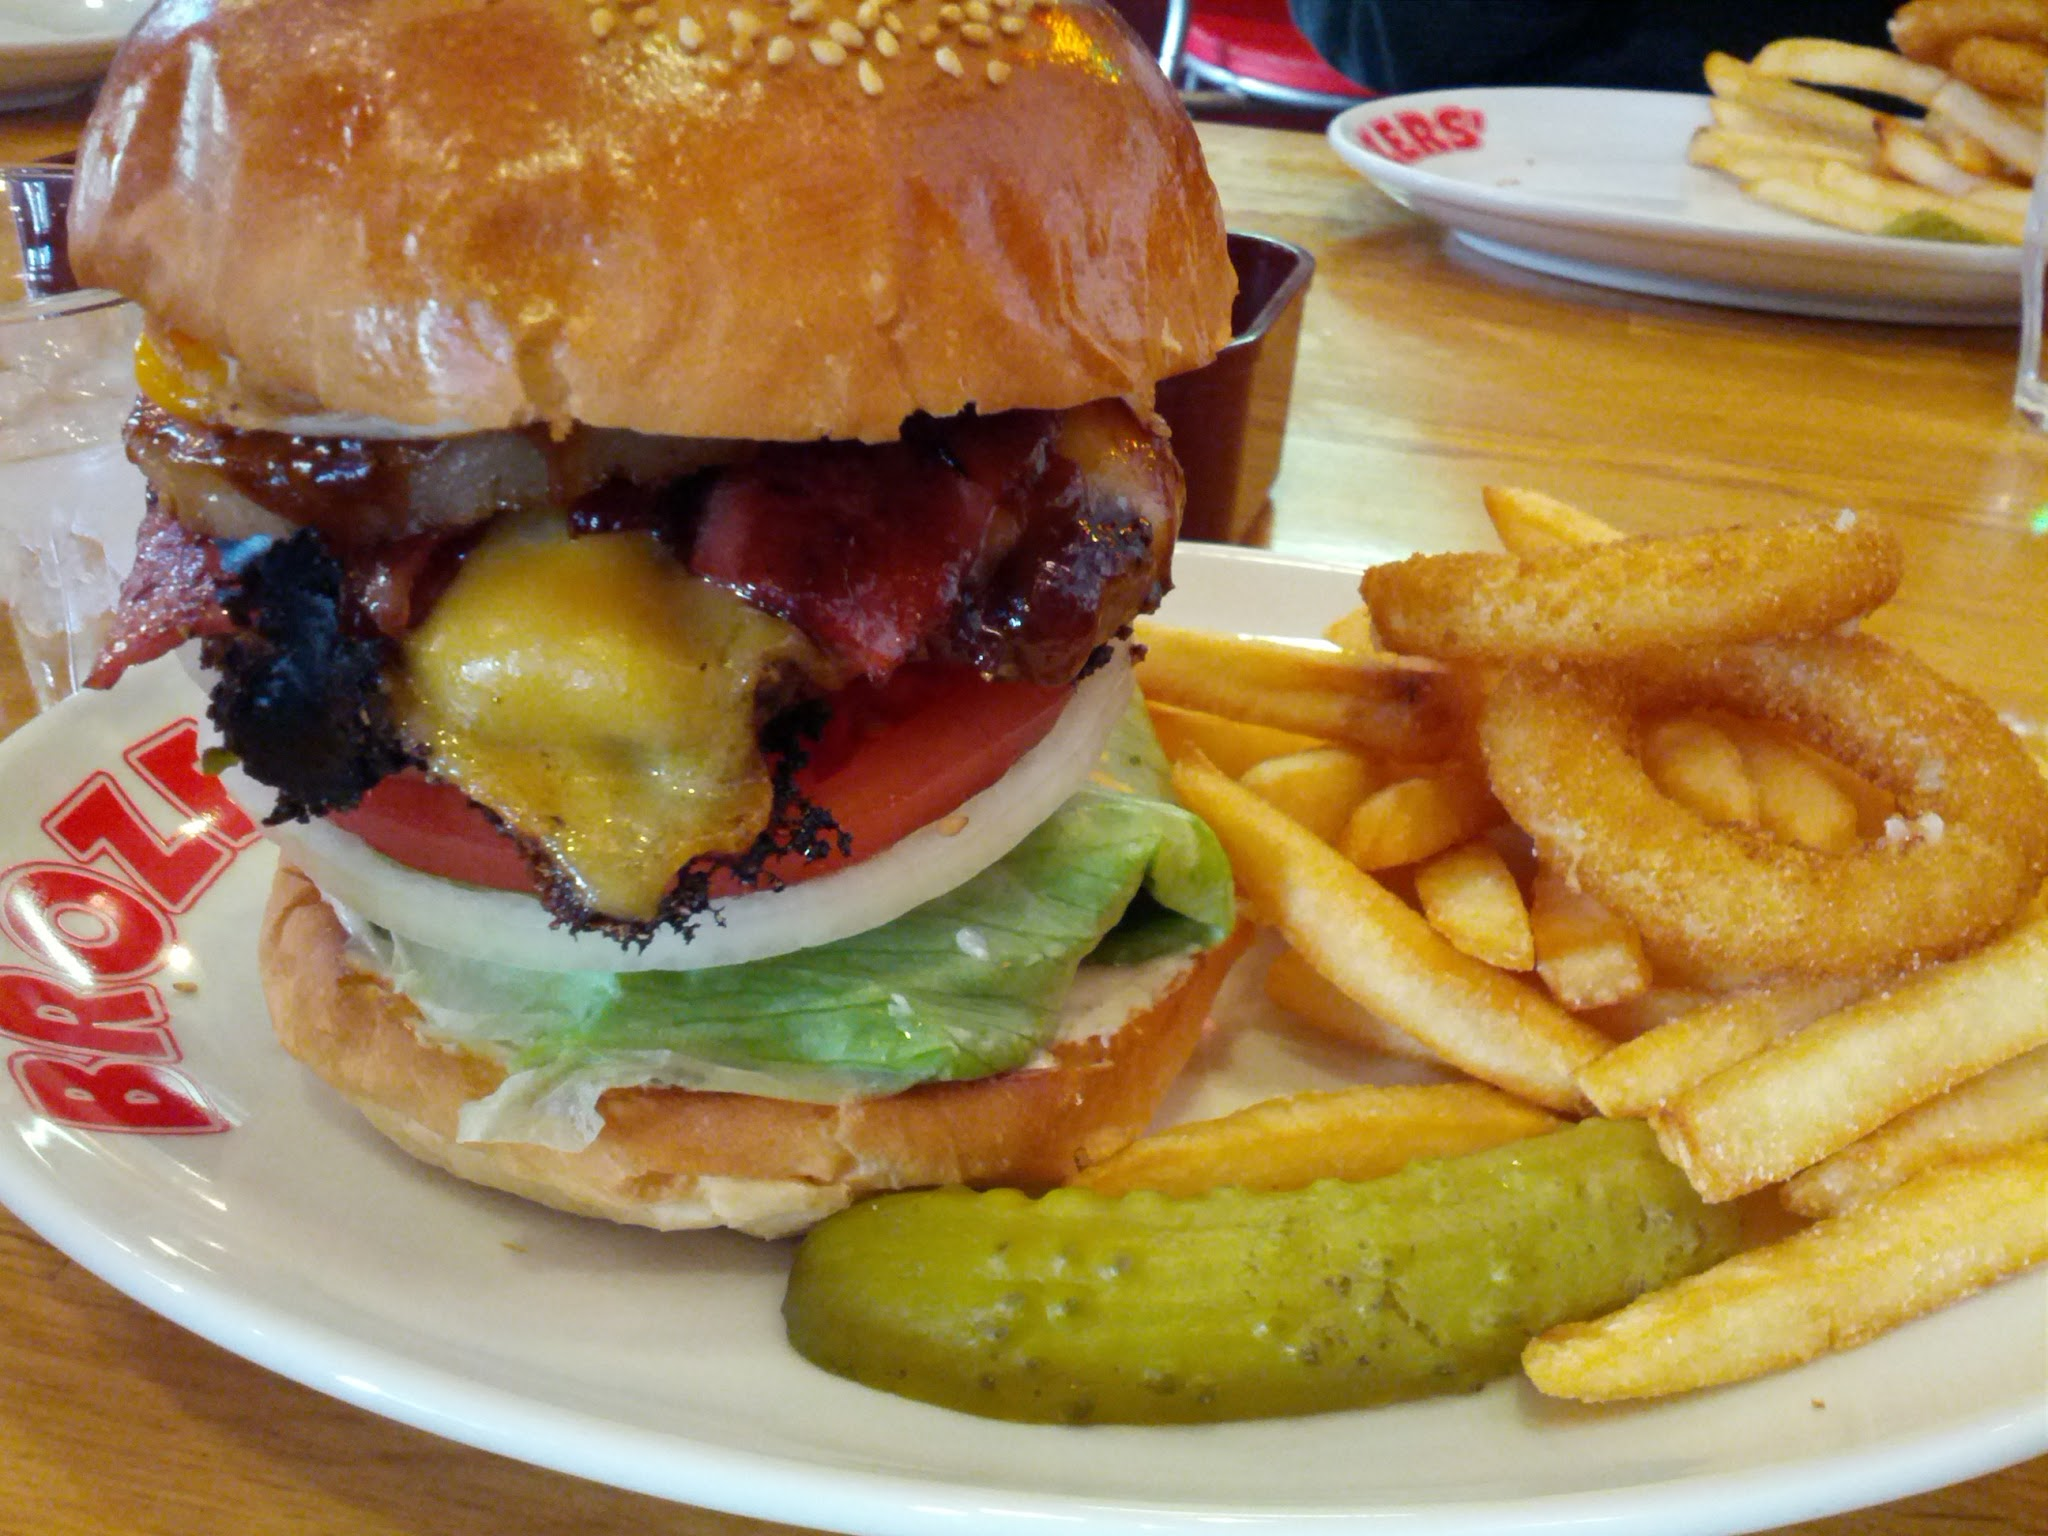
\includegraphics[width=0.6\textwidth]{../images/brozers.jpg}
  \caption{東京のうまいハンバーガー屋リストに度々名前が上がるブラザーズ 具材全てが肉厚で美味い}
\end{figure}

\begin{figure}[H]
  \centering
  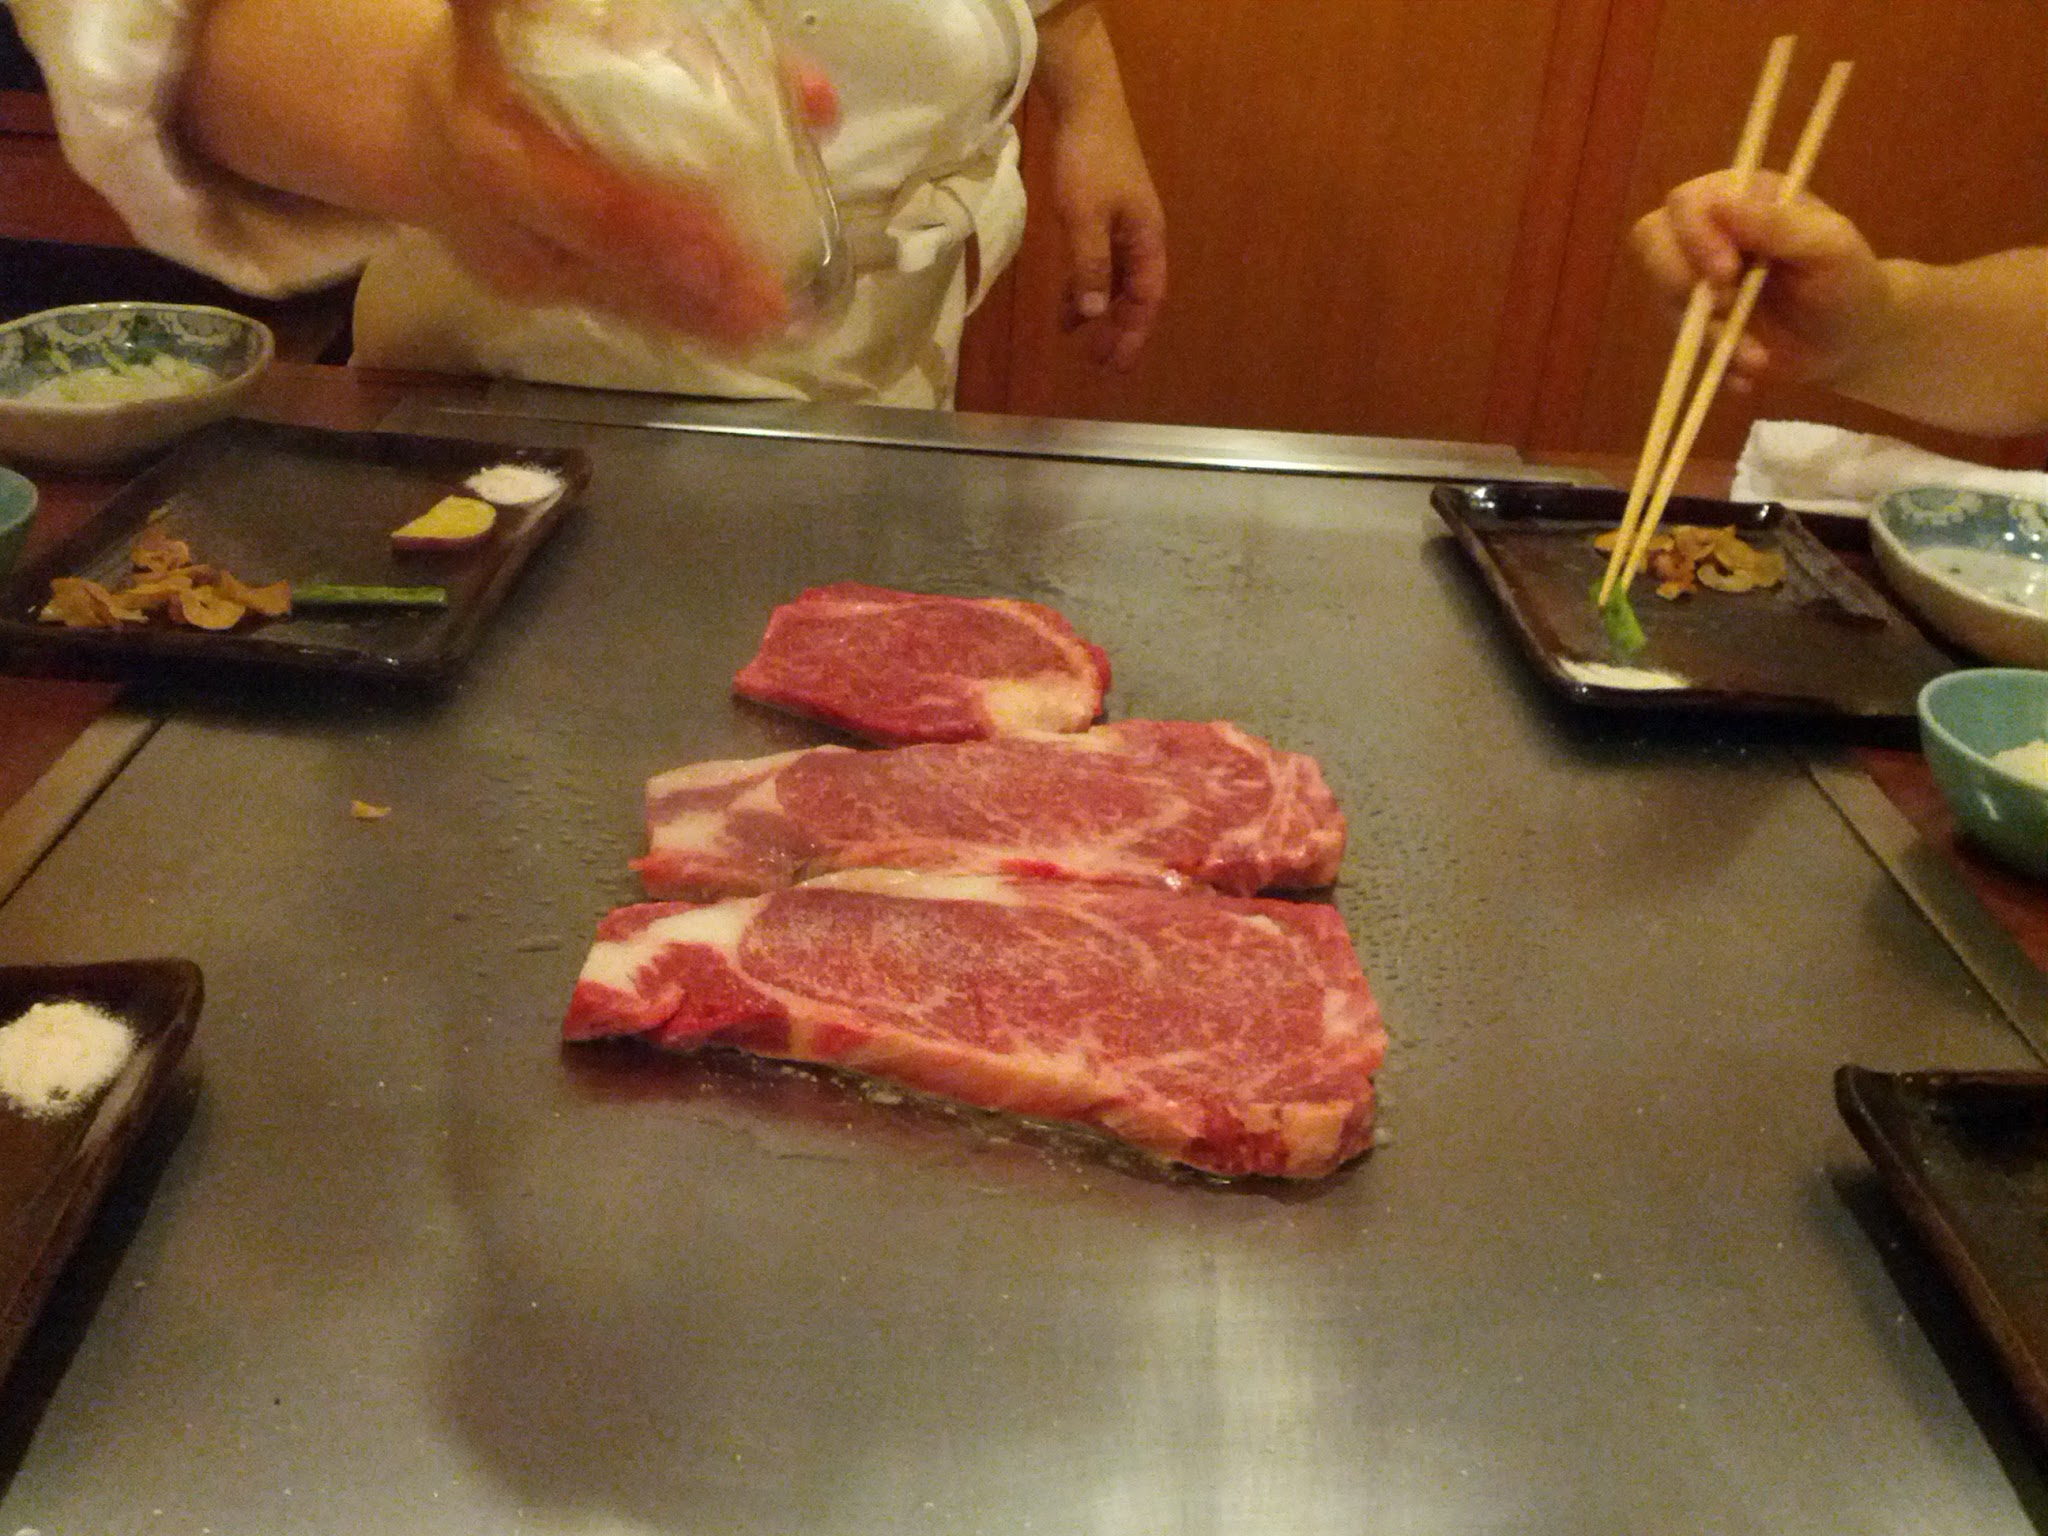
\includegraphics[width=0.6\textwidth]{../images/imahan.jpg}
  \caption{年に3日間だけの今半祭りはD社員が押し寄せる 肉爺が目の前でステーキを焼いてくれる}
\end{figure}

\begin{figure}[H]
  \centering
  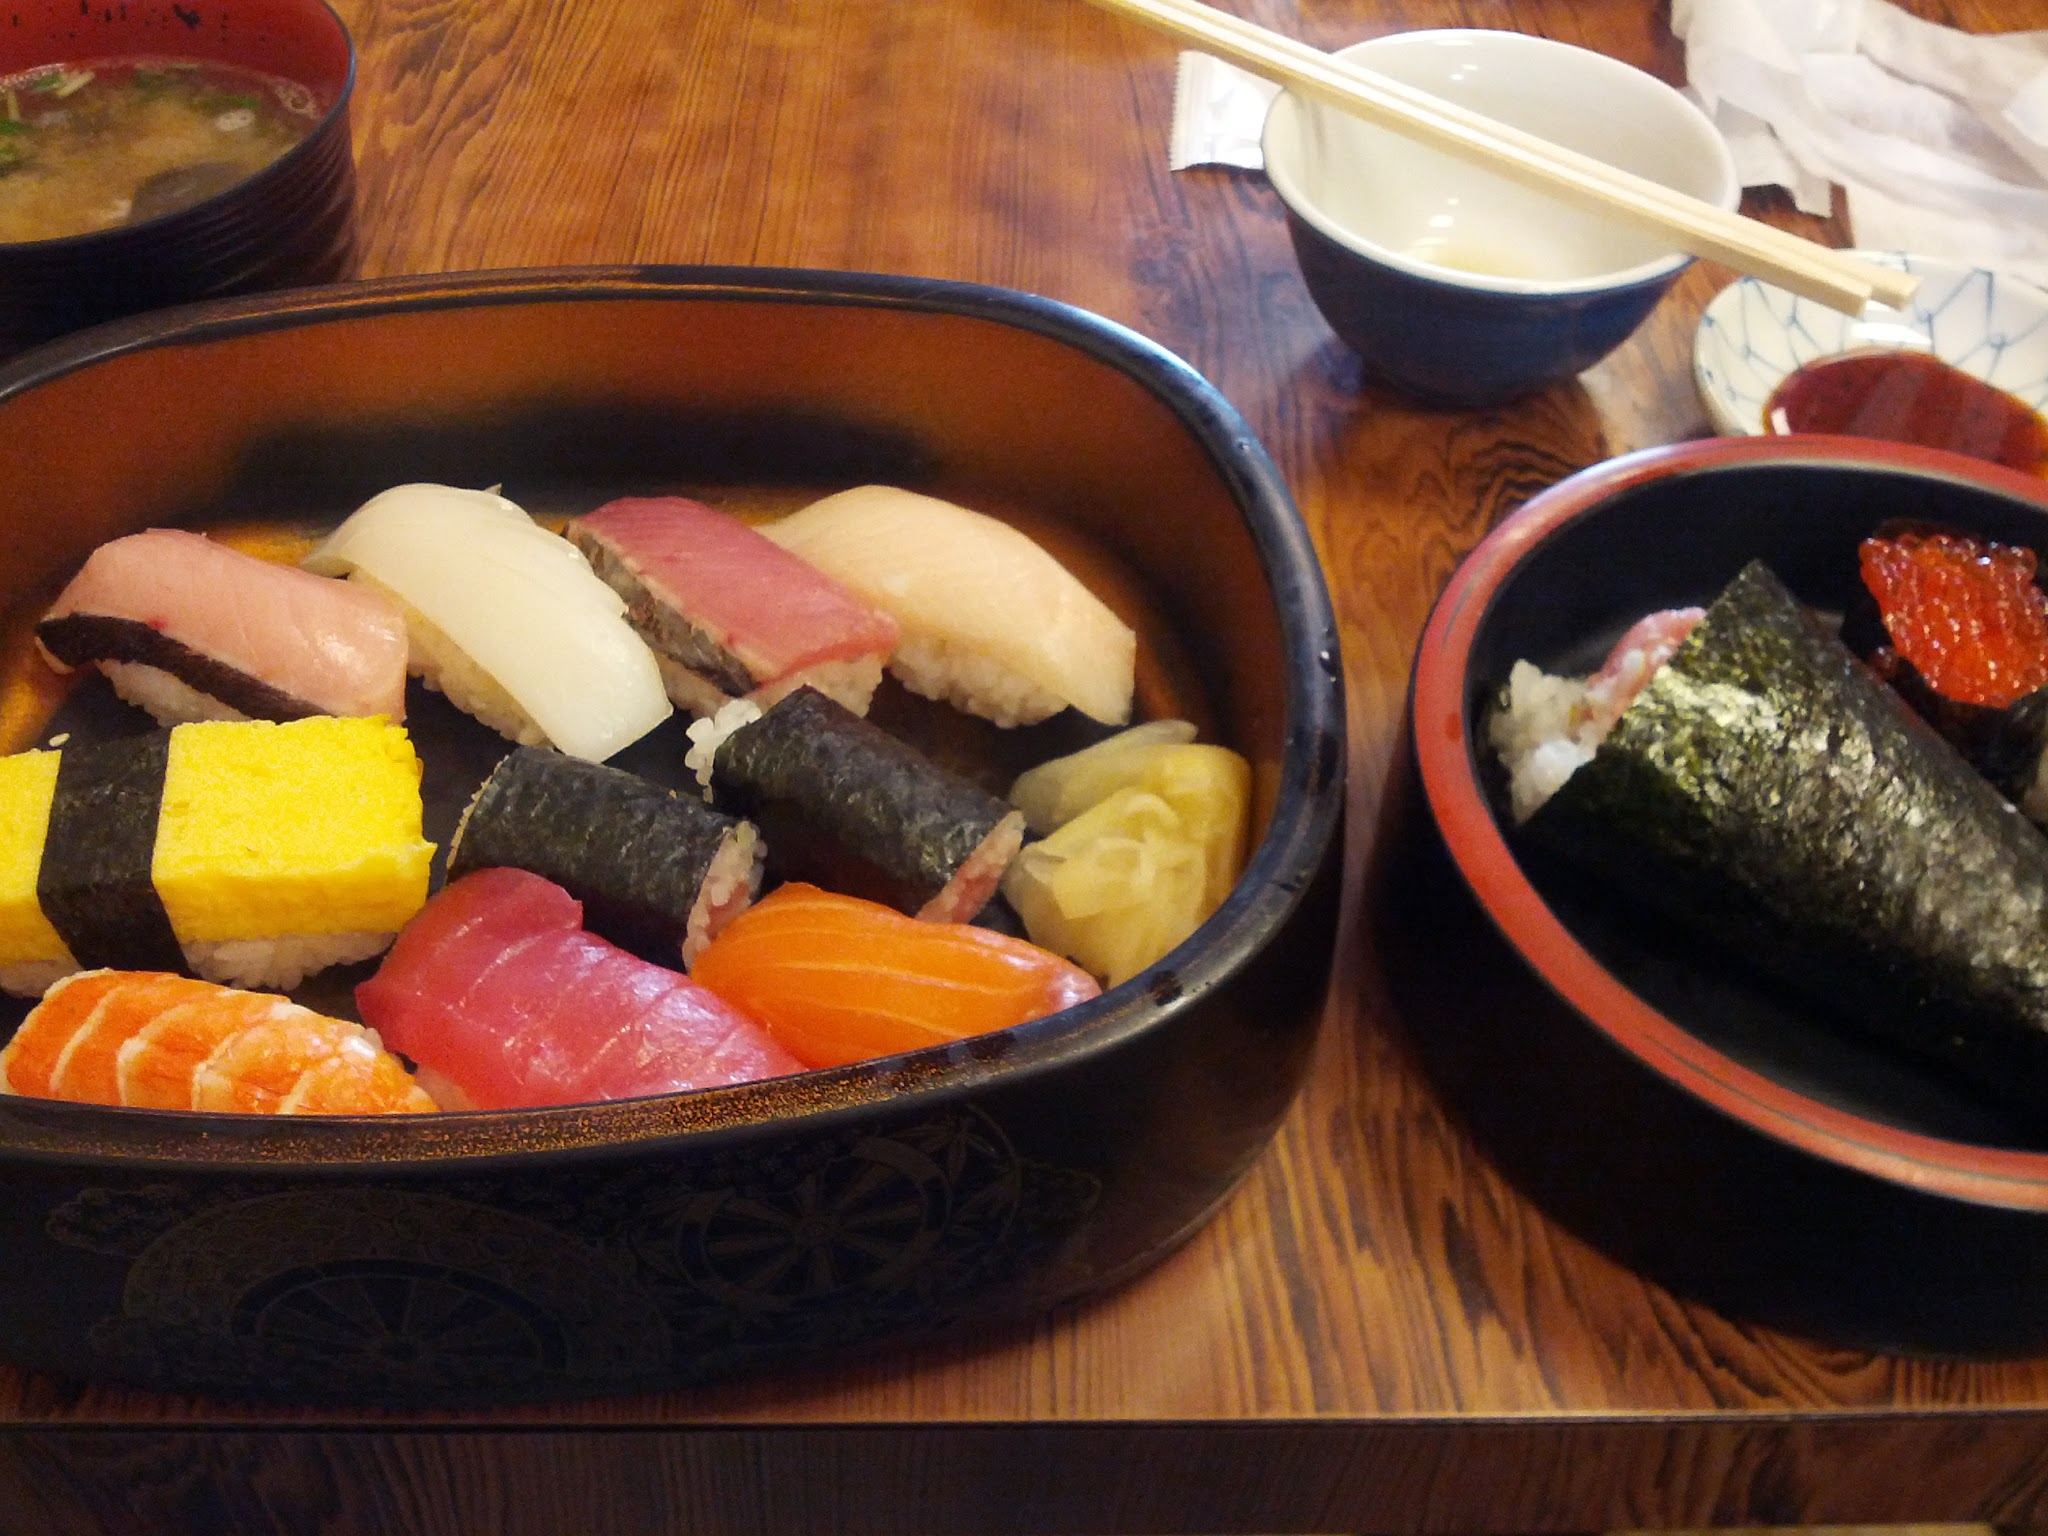
\includegraphics[width=0.5\textwidth]{../images/ittetsu.jpg}
  \caption{ちょっと豪華にシースーと言ったら一徹 といっても安くて美味くてボリュームもある}
\end{figure}

\begin{figure}[H]
  \centering
  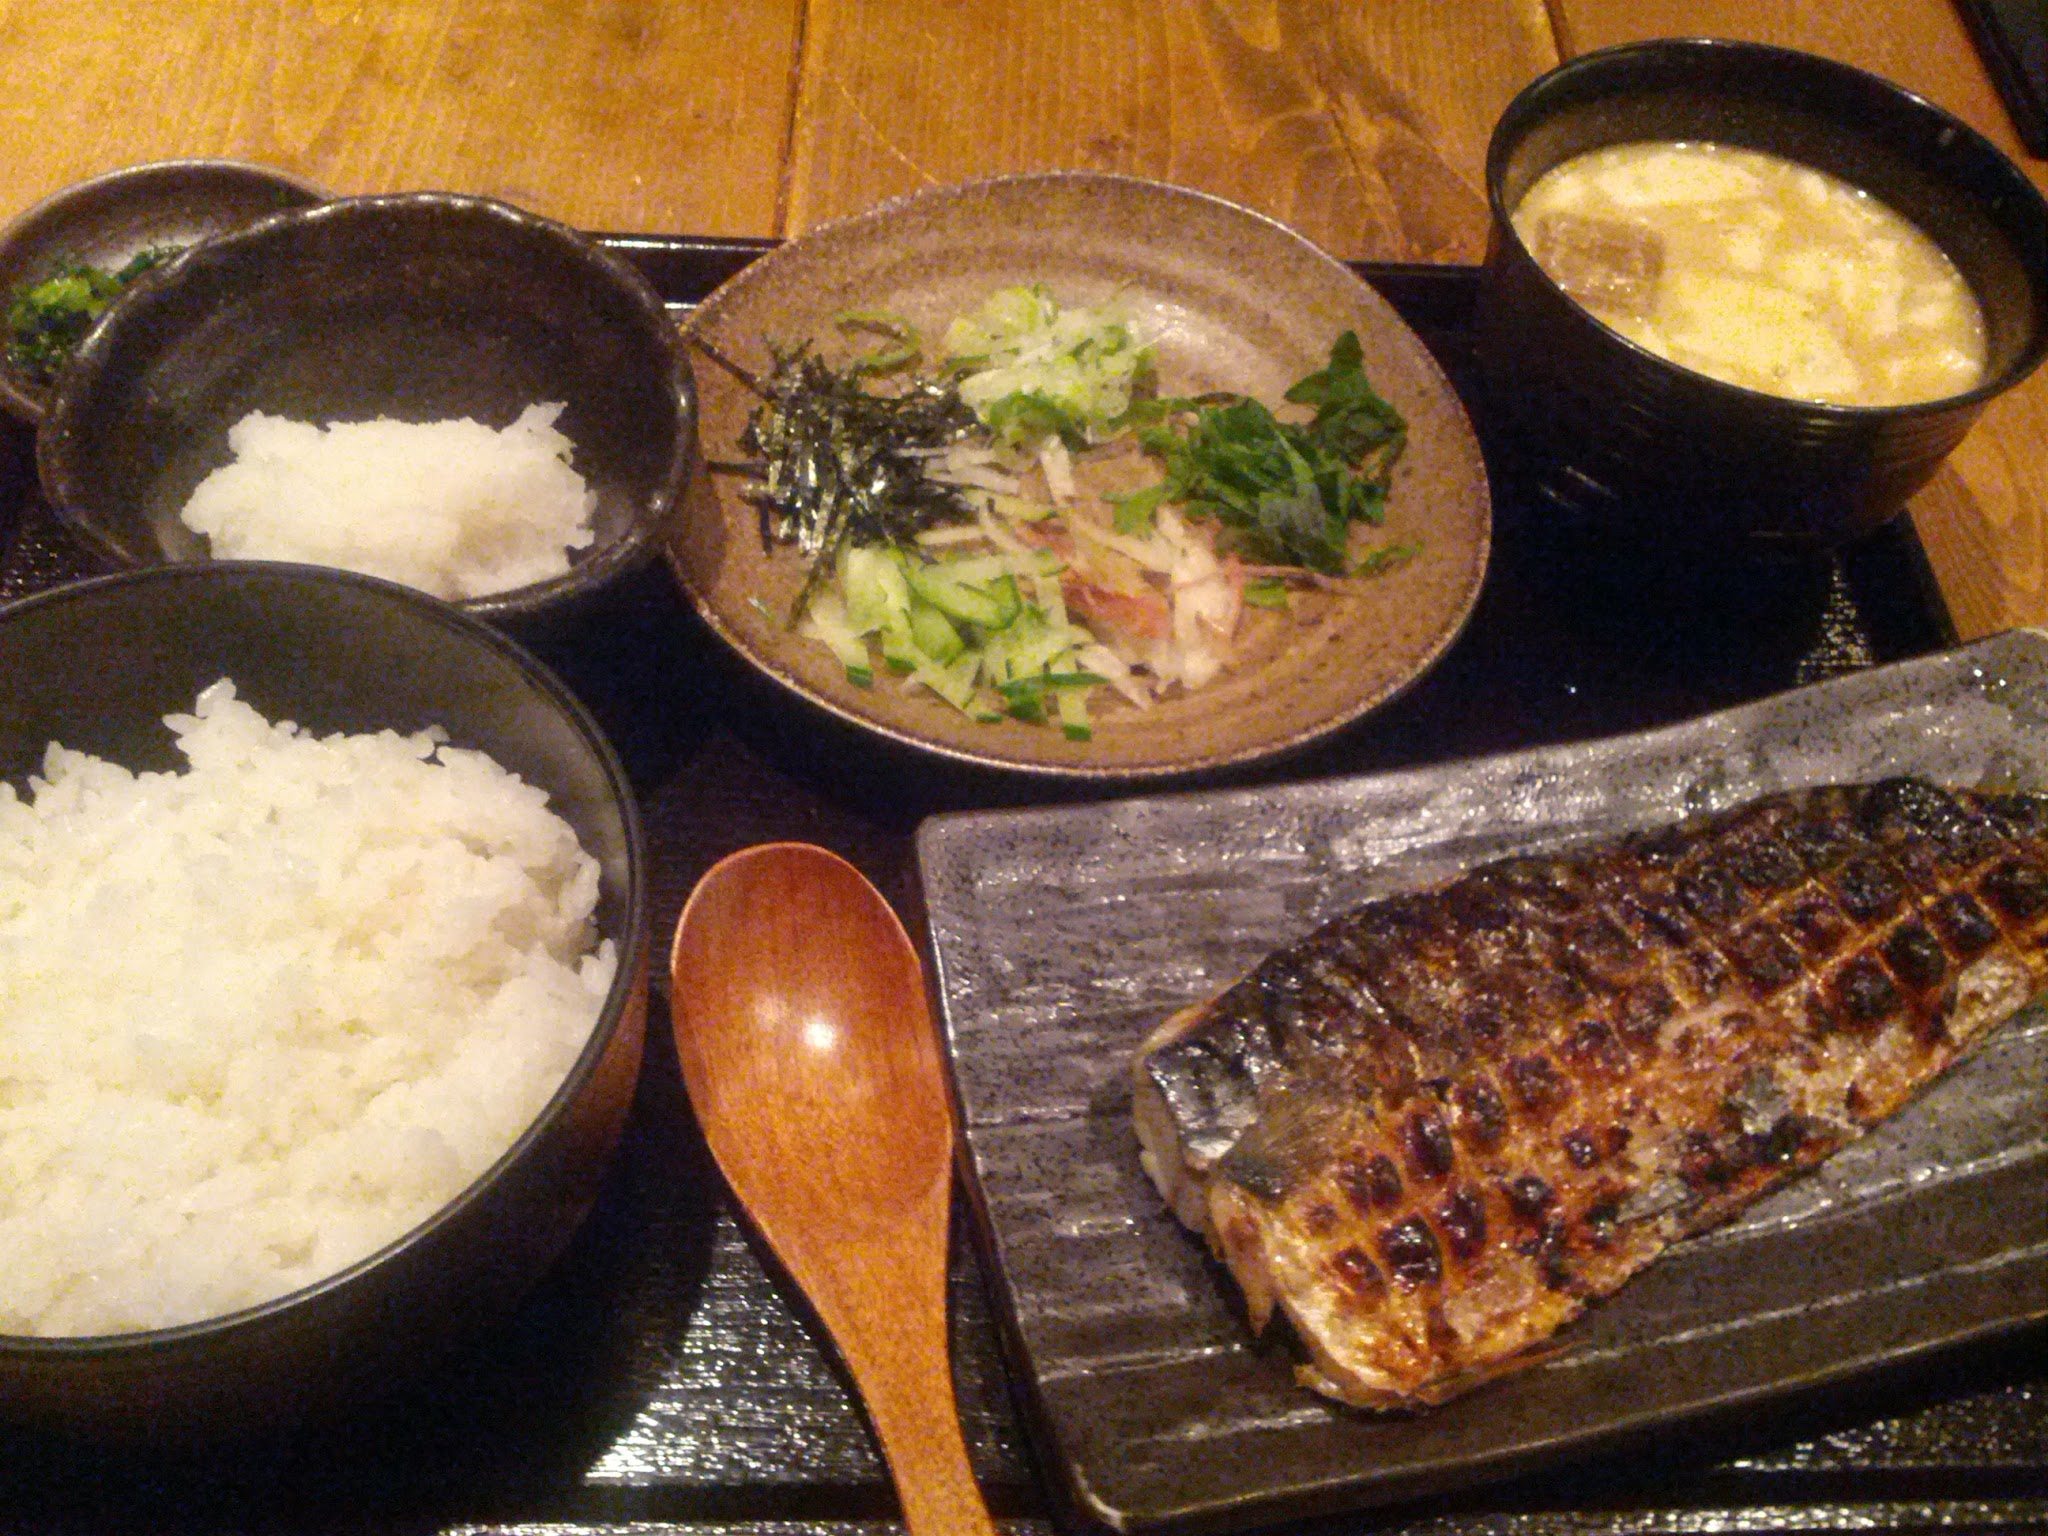
\includegraphics[width=0.5\textwidth]{../images/marushow.jpg}
  \caption{築地が近いから魚も美味い 丸正 夏限定の冷や汁が絶品}
\end{figure}

\begin{figure}[H]
  \centering
  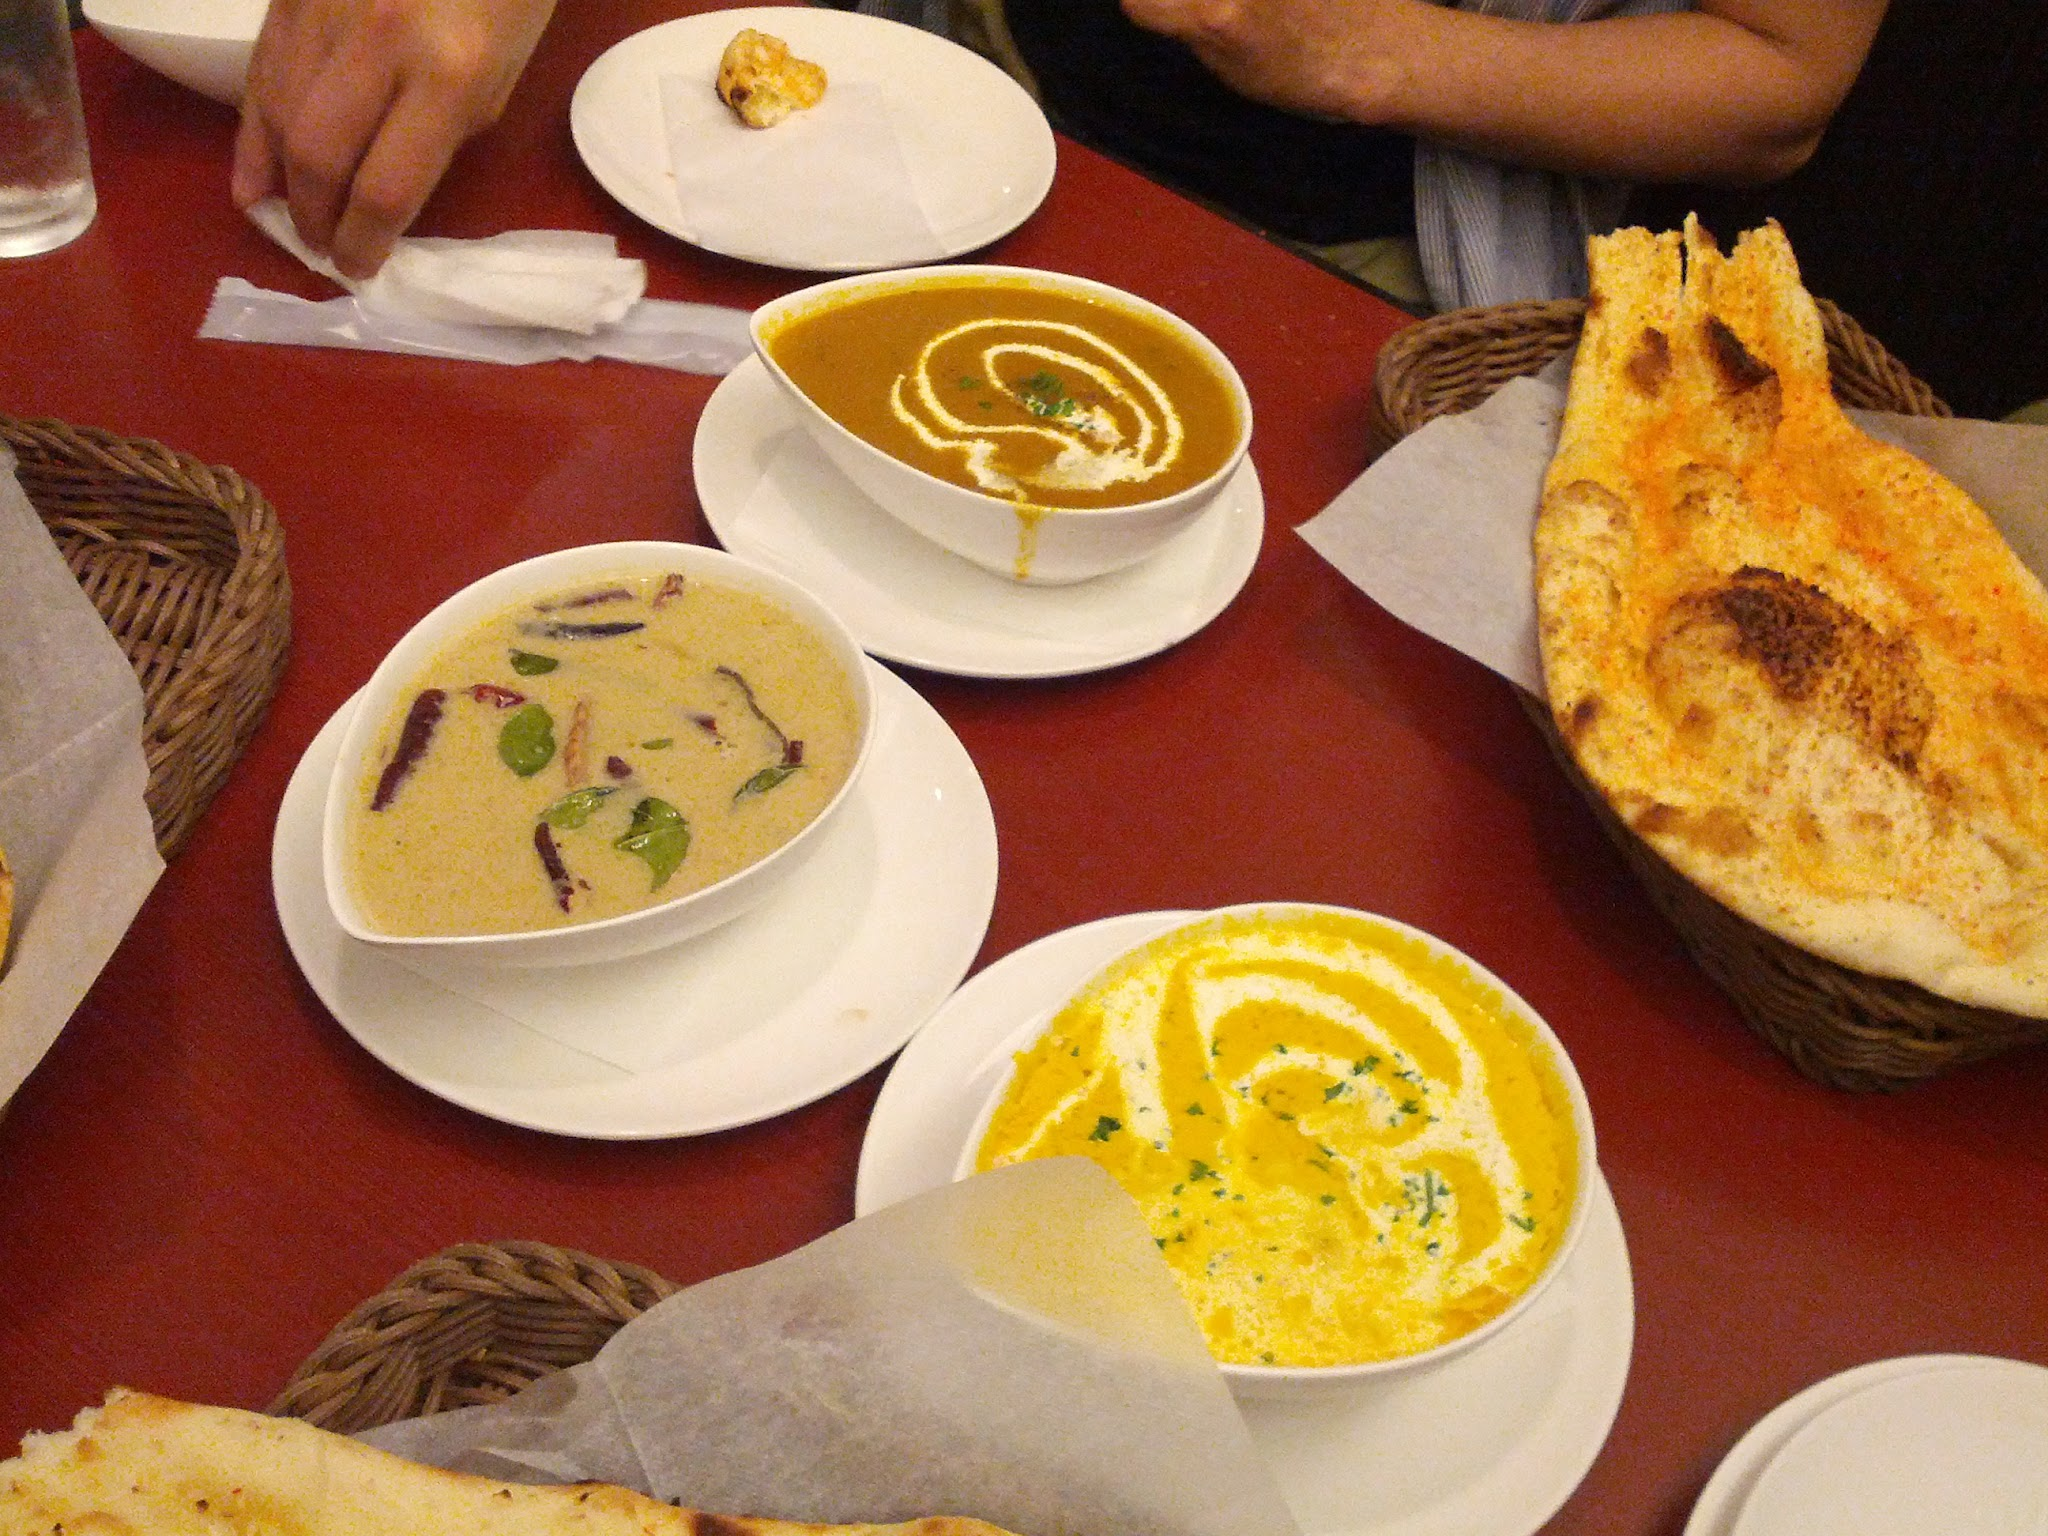
\includegraphics[width=0.5\textwidth]{../images/ganeza.jpg}
  \caption{明治座の目の前にあるカレーのガネーシャ 適当に頼んでシェアして食う なぜかとんかつとナシゴレンが美味い}
\end{figure}

\begin{figure}[H]
  \centering
  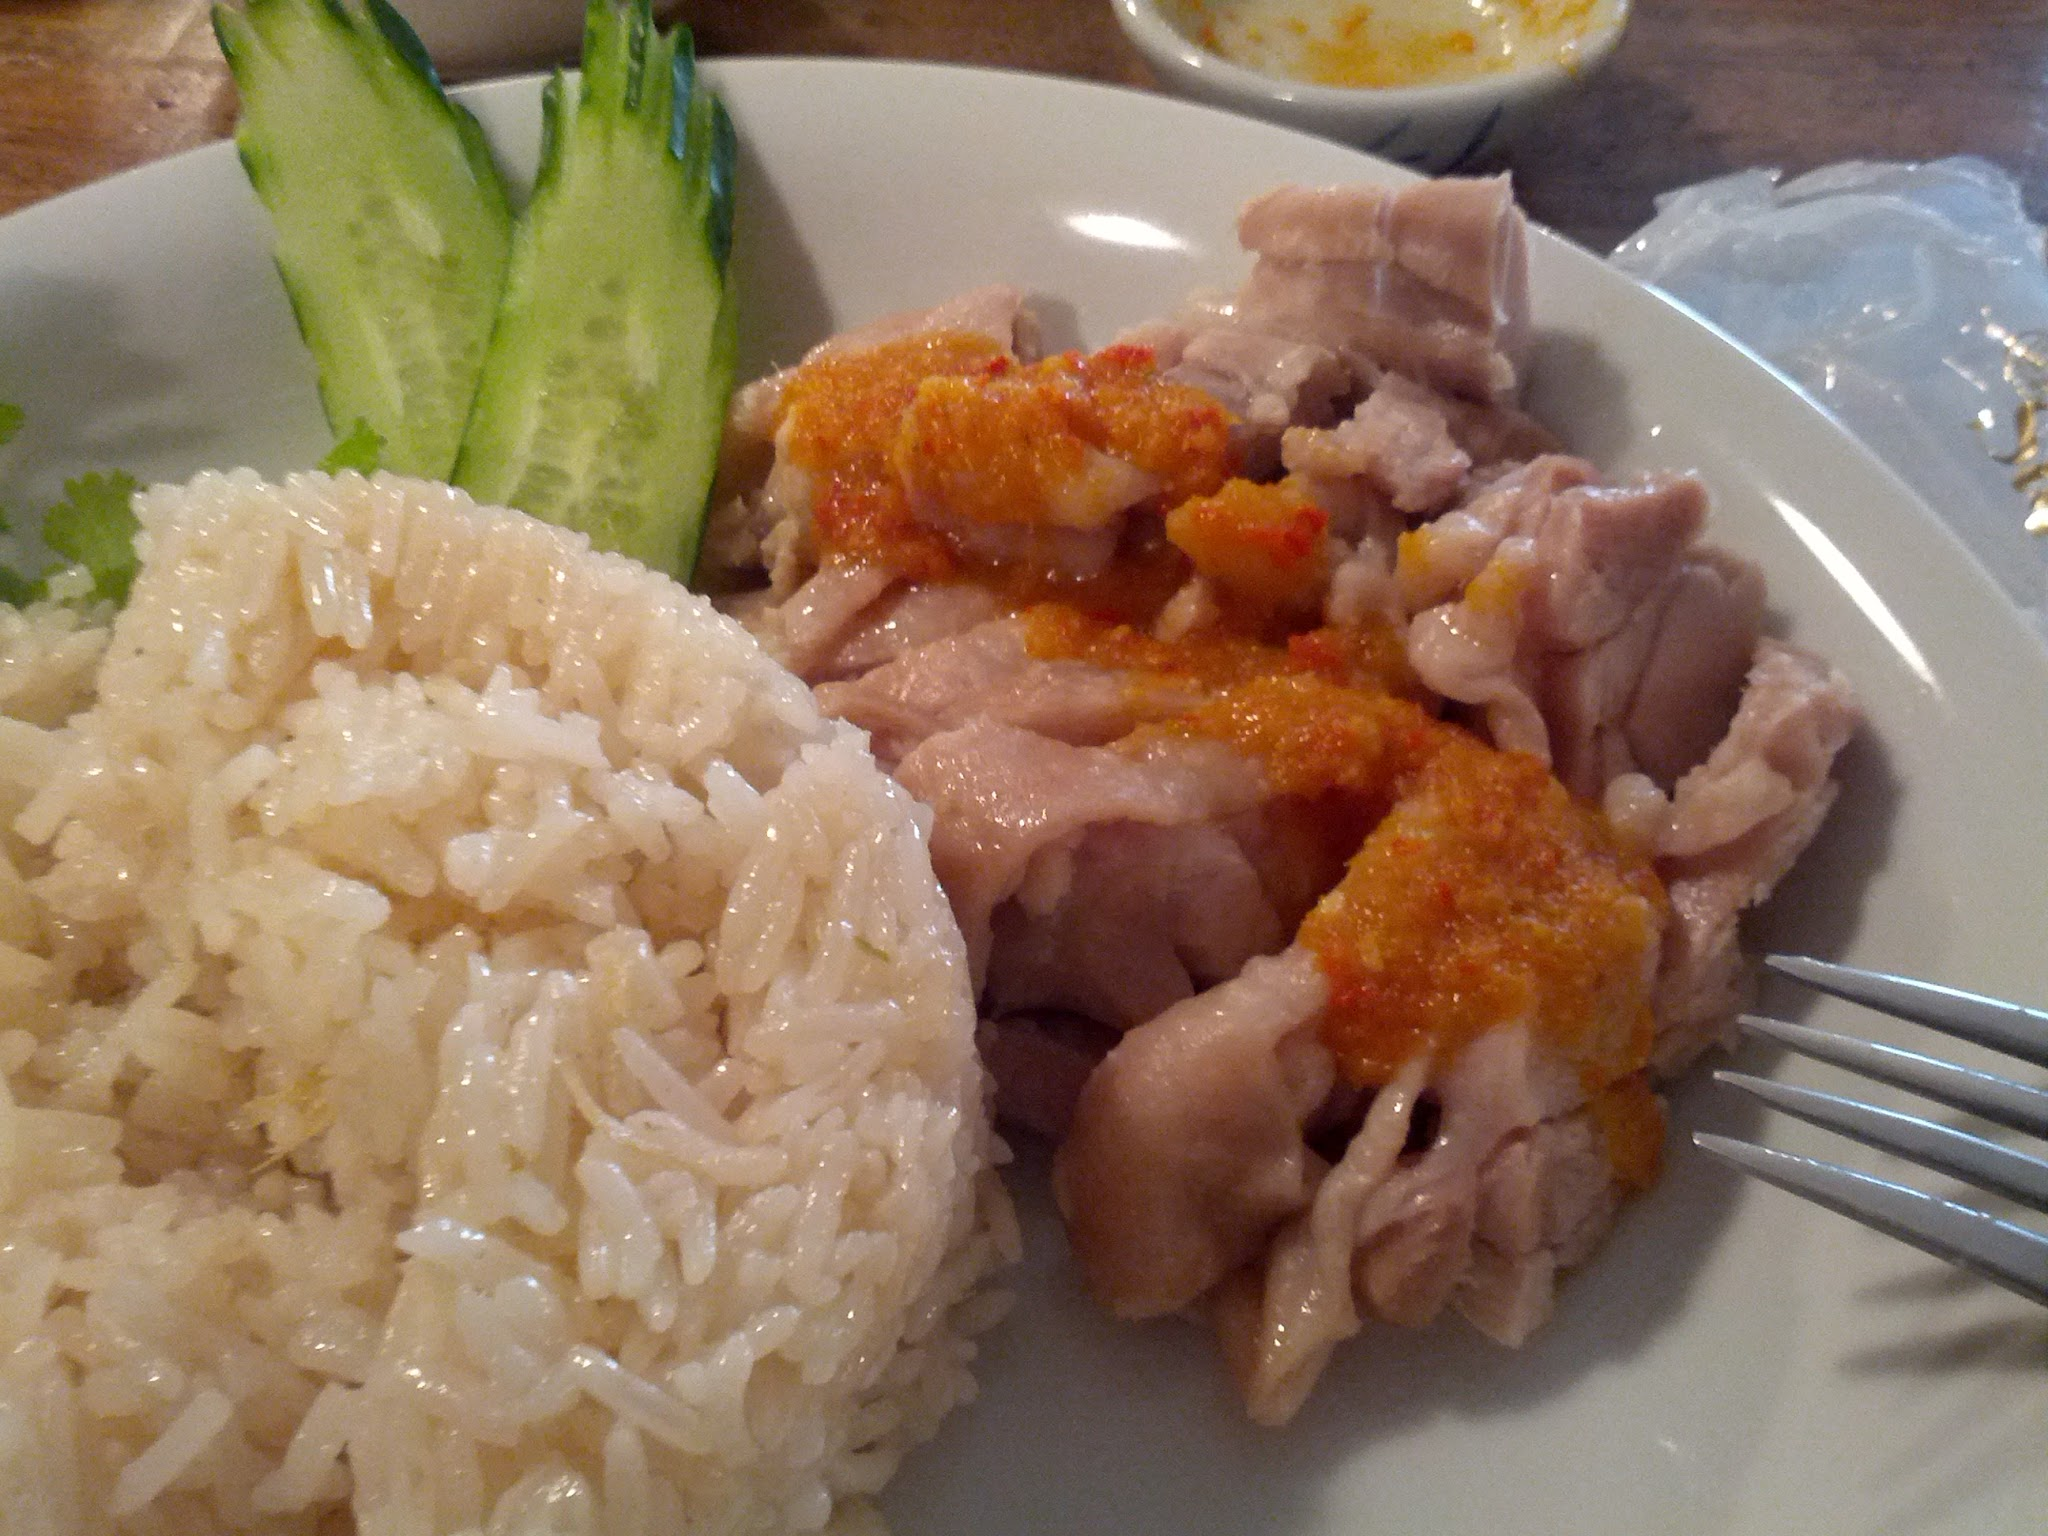
\includegraphics[width=0.5\textwidth]{../images/rarara.jpg}
  \caption{他の客は女子だらけ タイを中心としたアジア料理のラララ食堂 姉妹店増殖中 銀座にも来てほしい}
\end{figure}

\begin{figure}[H]
  \centering
  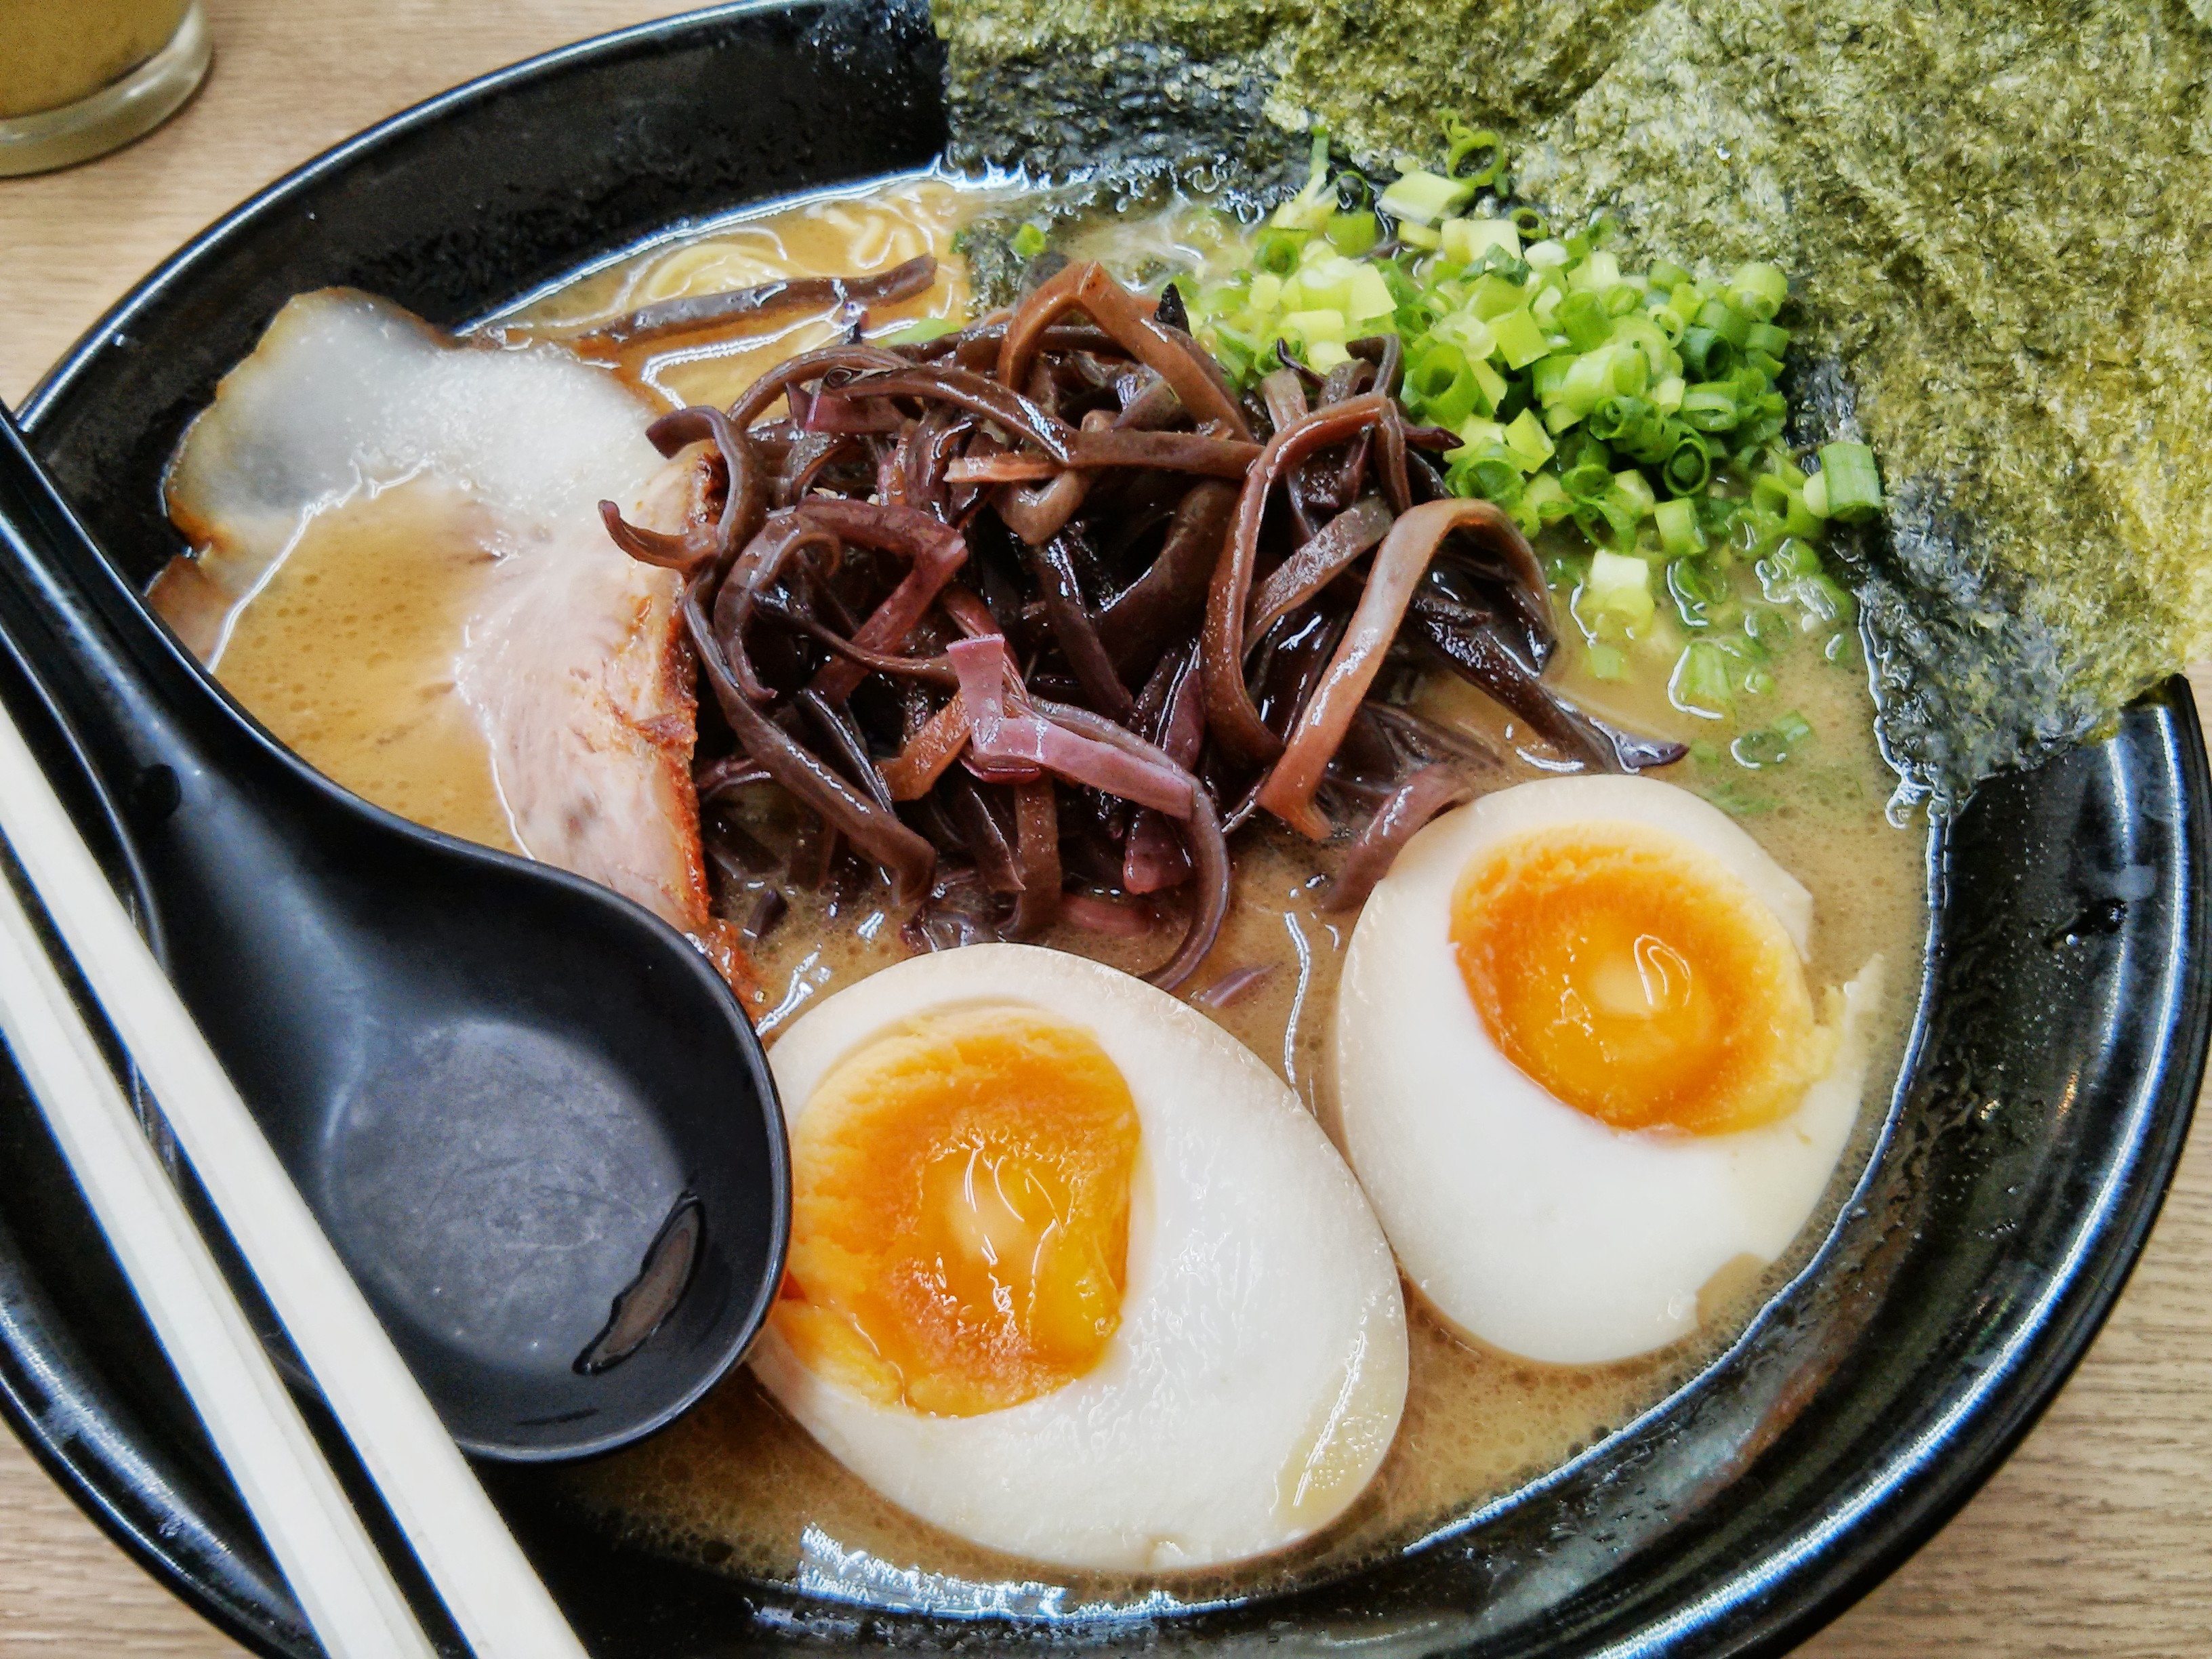
\includegraphics[width=0.5\textwidth]{../images/seiya.jpg}
  \caption{深夜までやってて重宝する 野菜たっぷりのラーメン せいや}
\end{figure}

\begin{figure}[H]
  \centering
  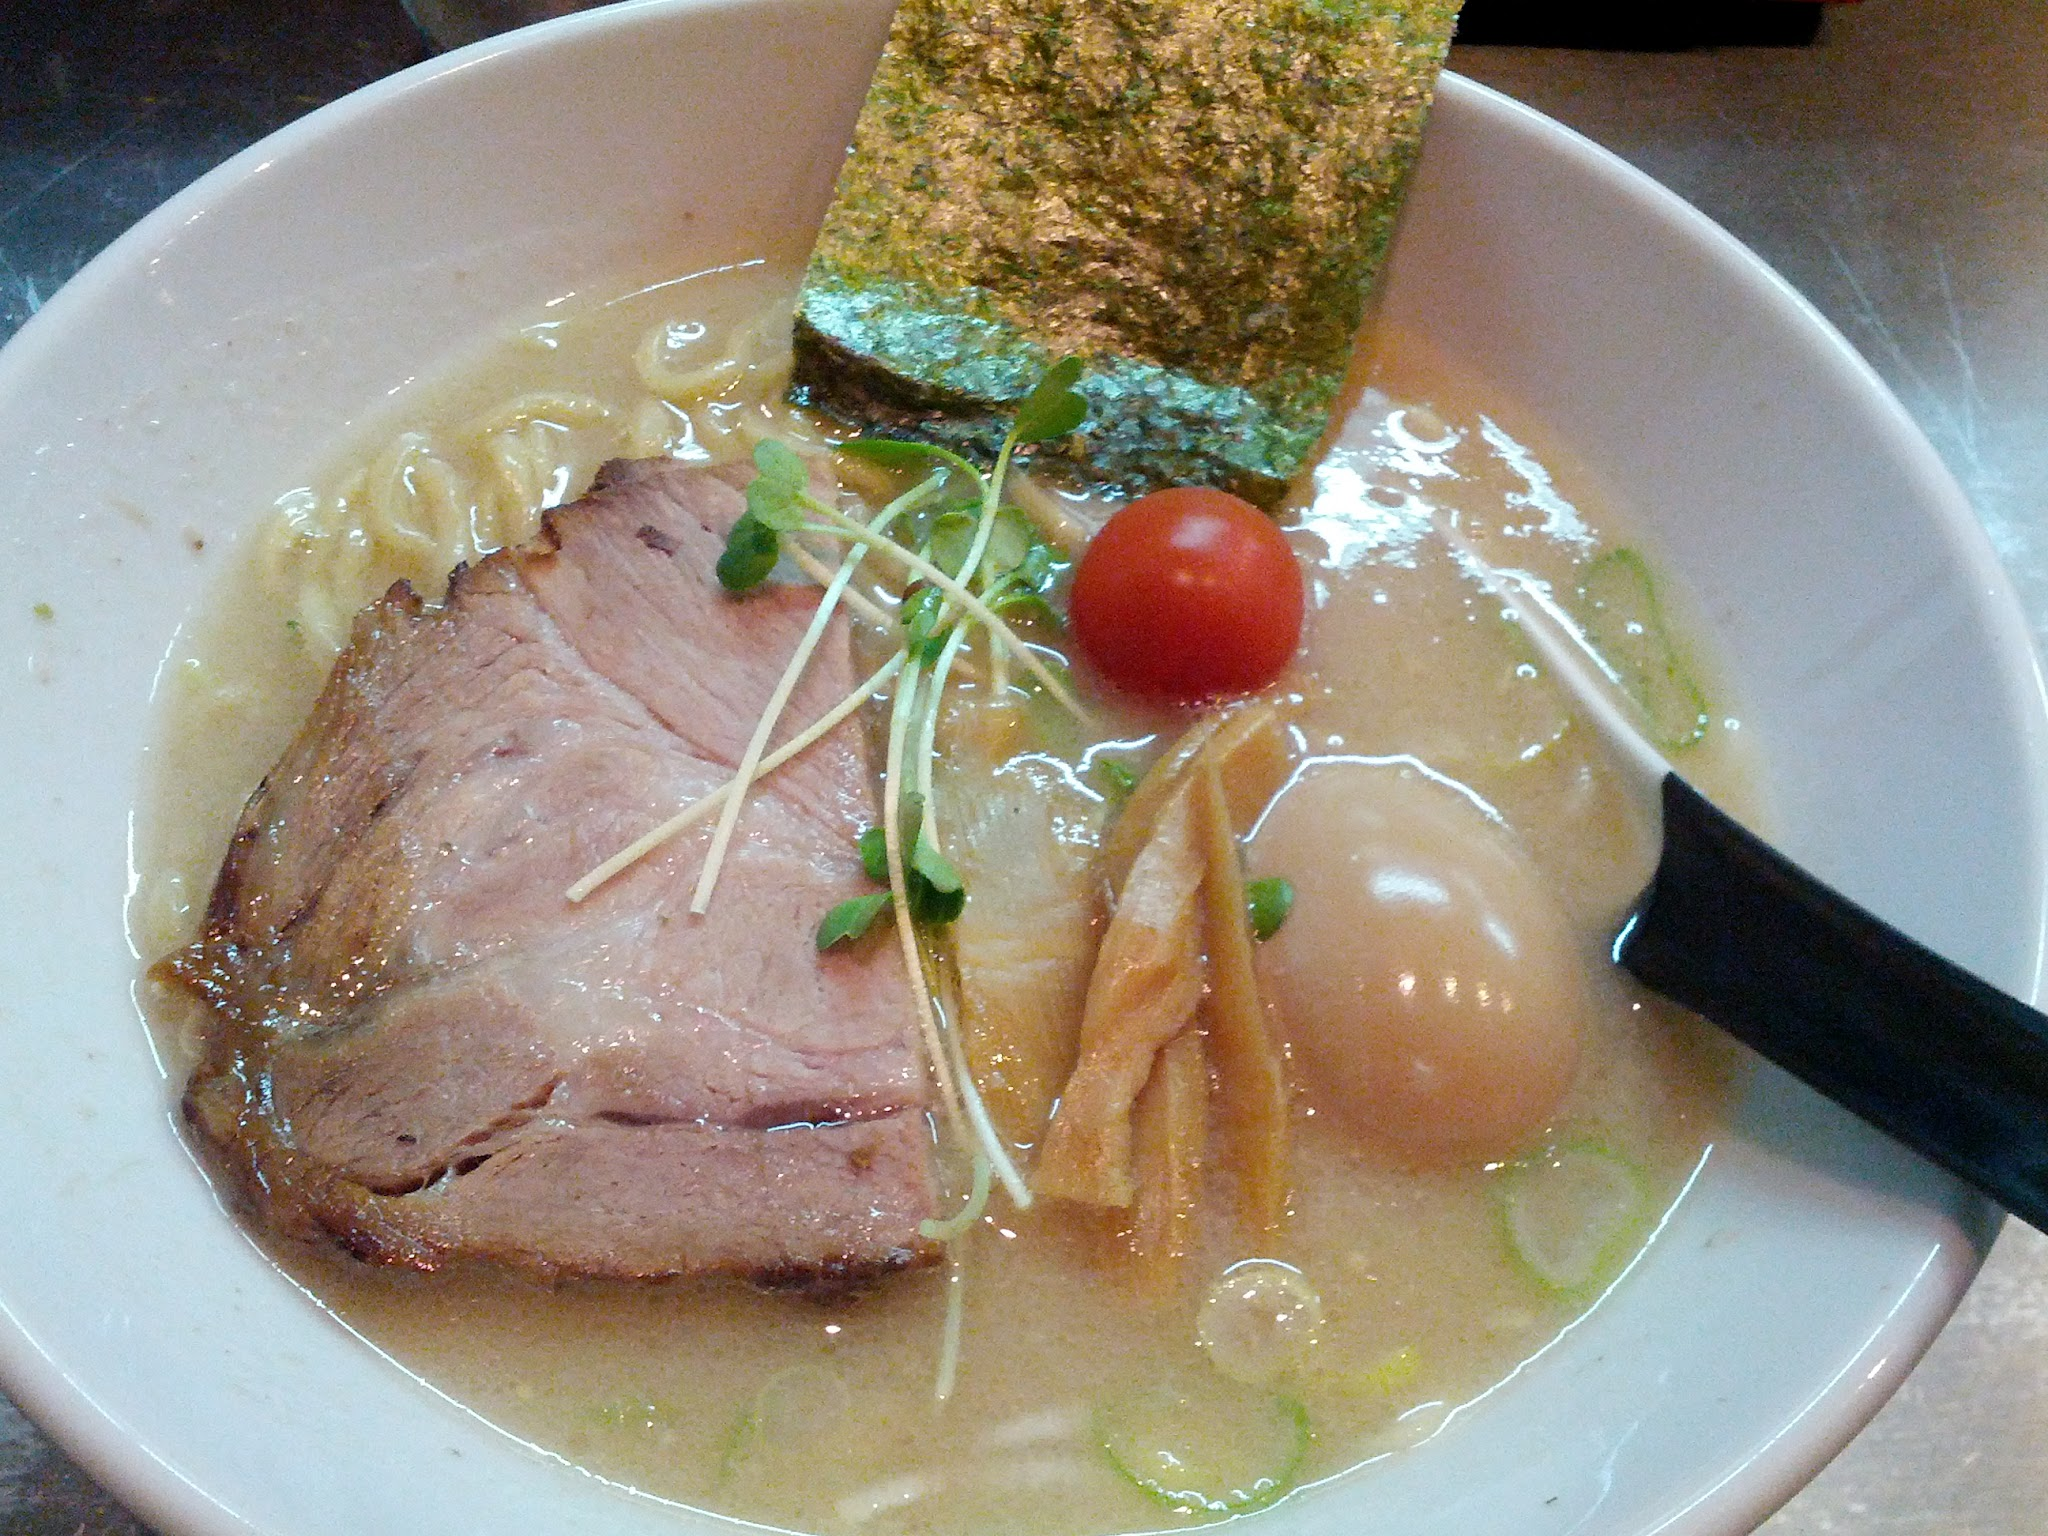
\includegraphics[width=0.5\textwidth]{../images/yamara.jpg}
  \caption{スープが旨すぎて全部飲んでも飲み足りない やまらぁ}
\end{figure}

\begin{figure}[H]
  \centering
  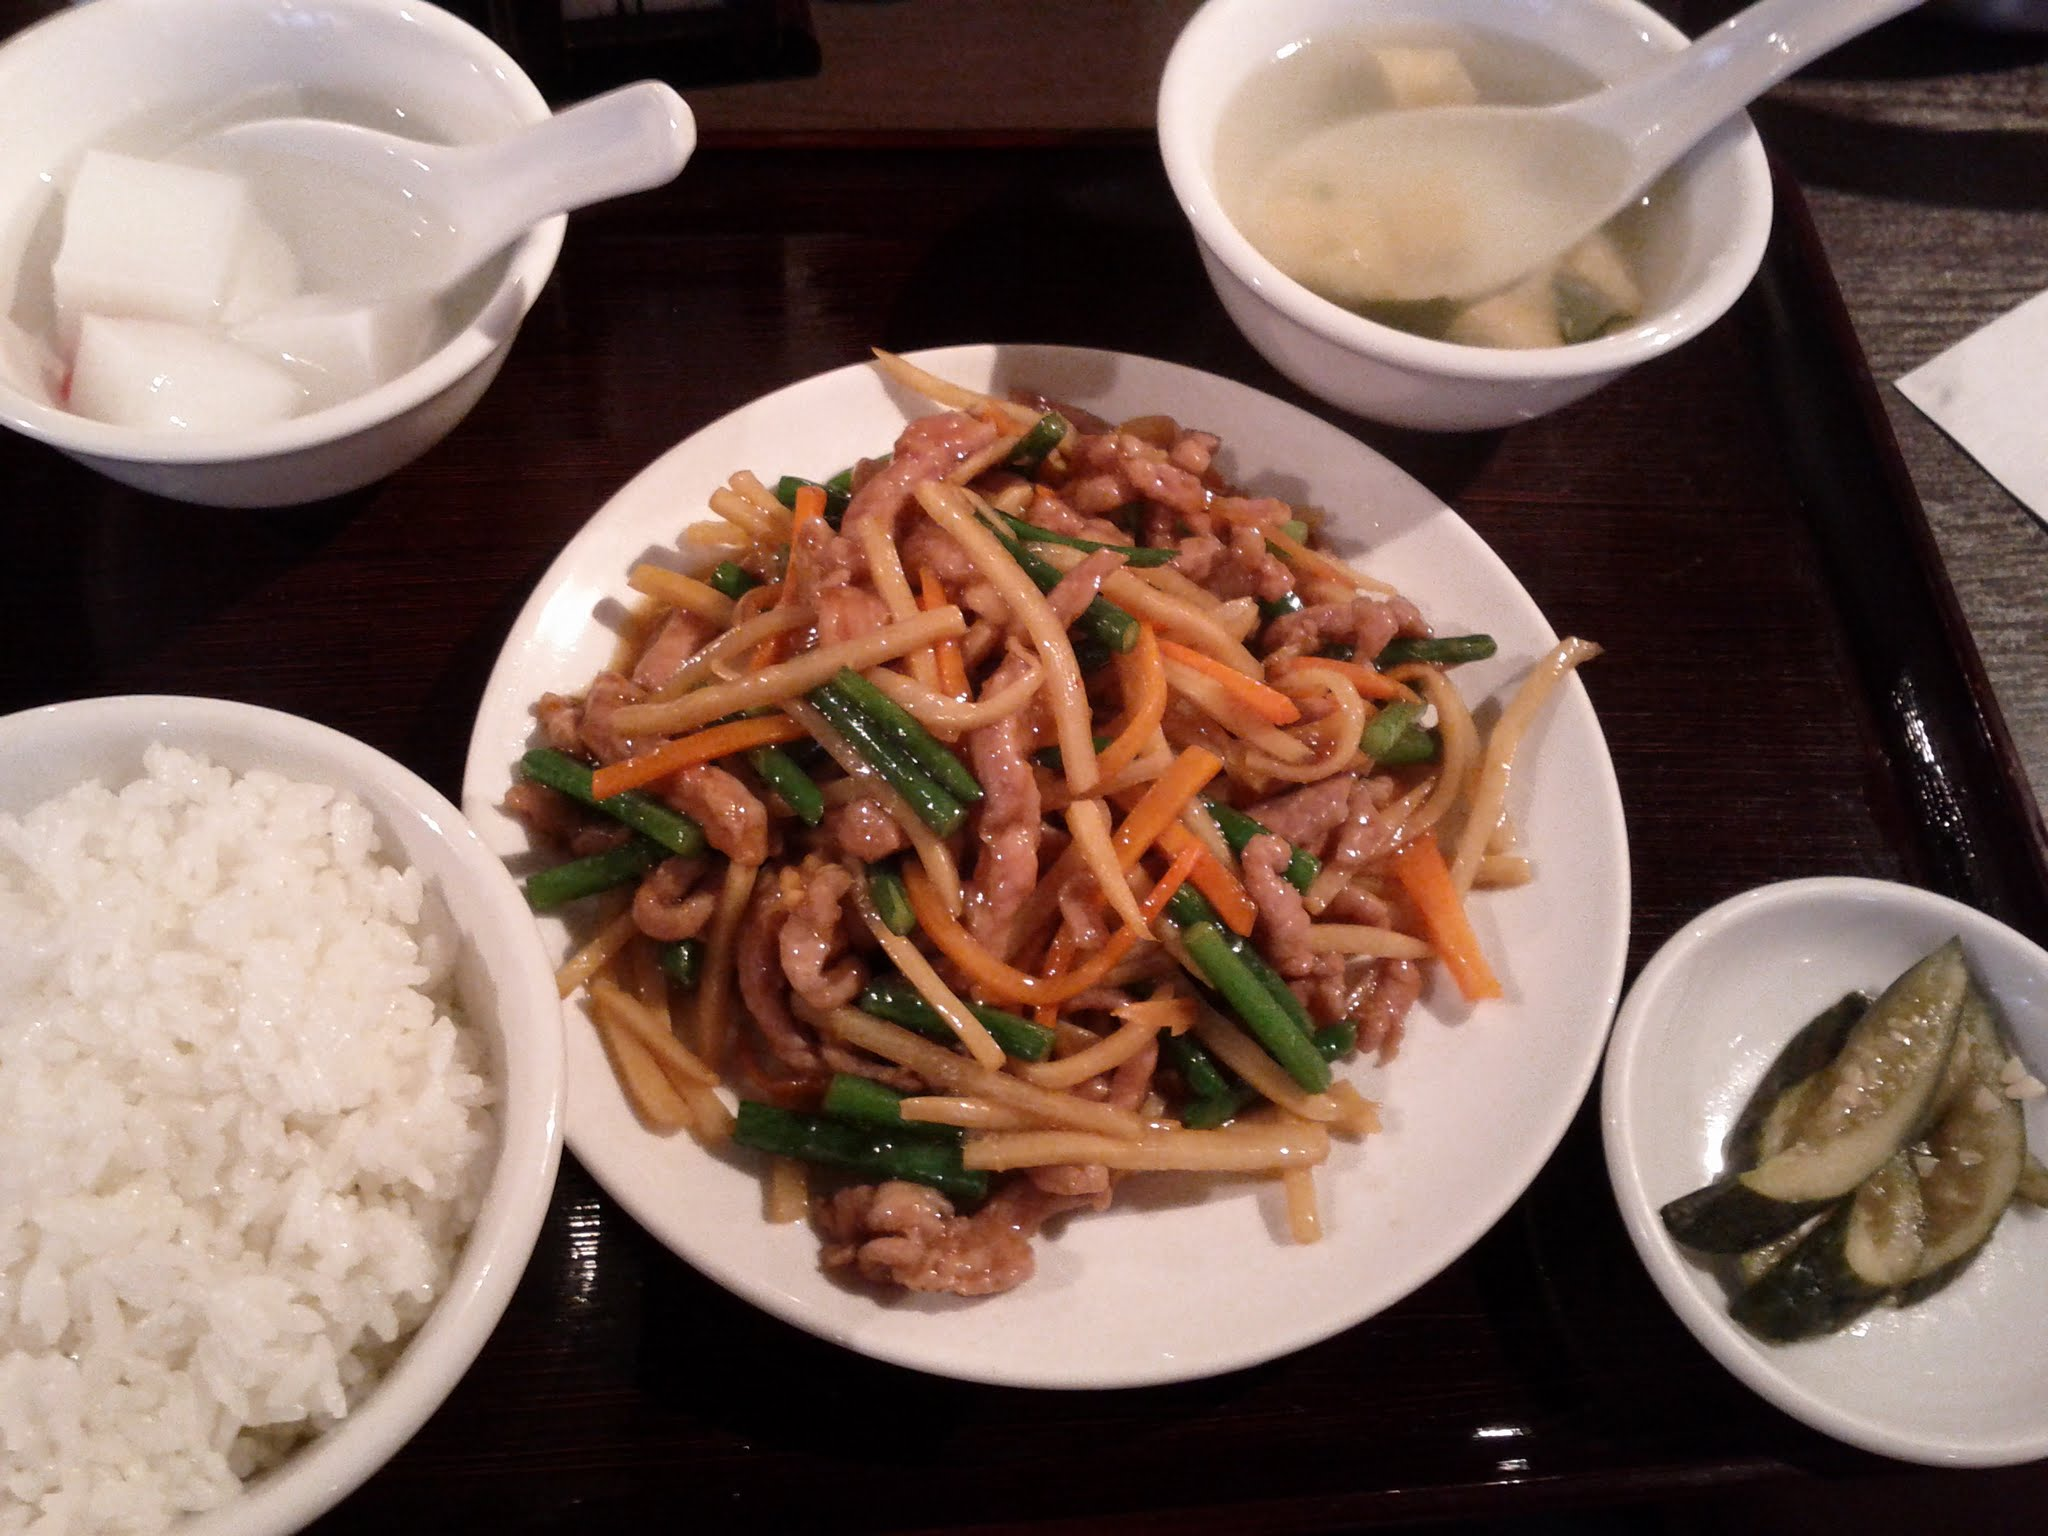
\includegraphics[width=0.5\textwidth]{../images/seigyo.jpg}
  \caption{量も味も罪である 中華料理の成暁 たまにごはんの代わりにチャーハンが出てくる}
\end{figure}

\begin{figure}[H]
  \centering
  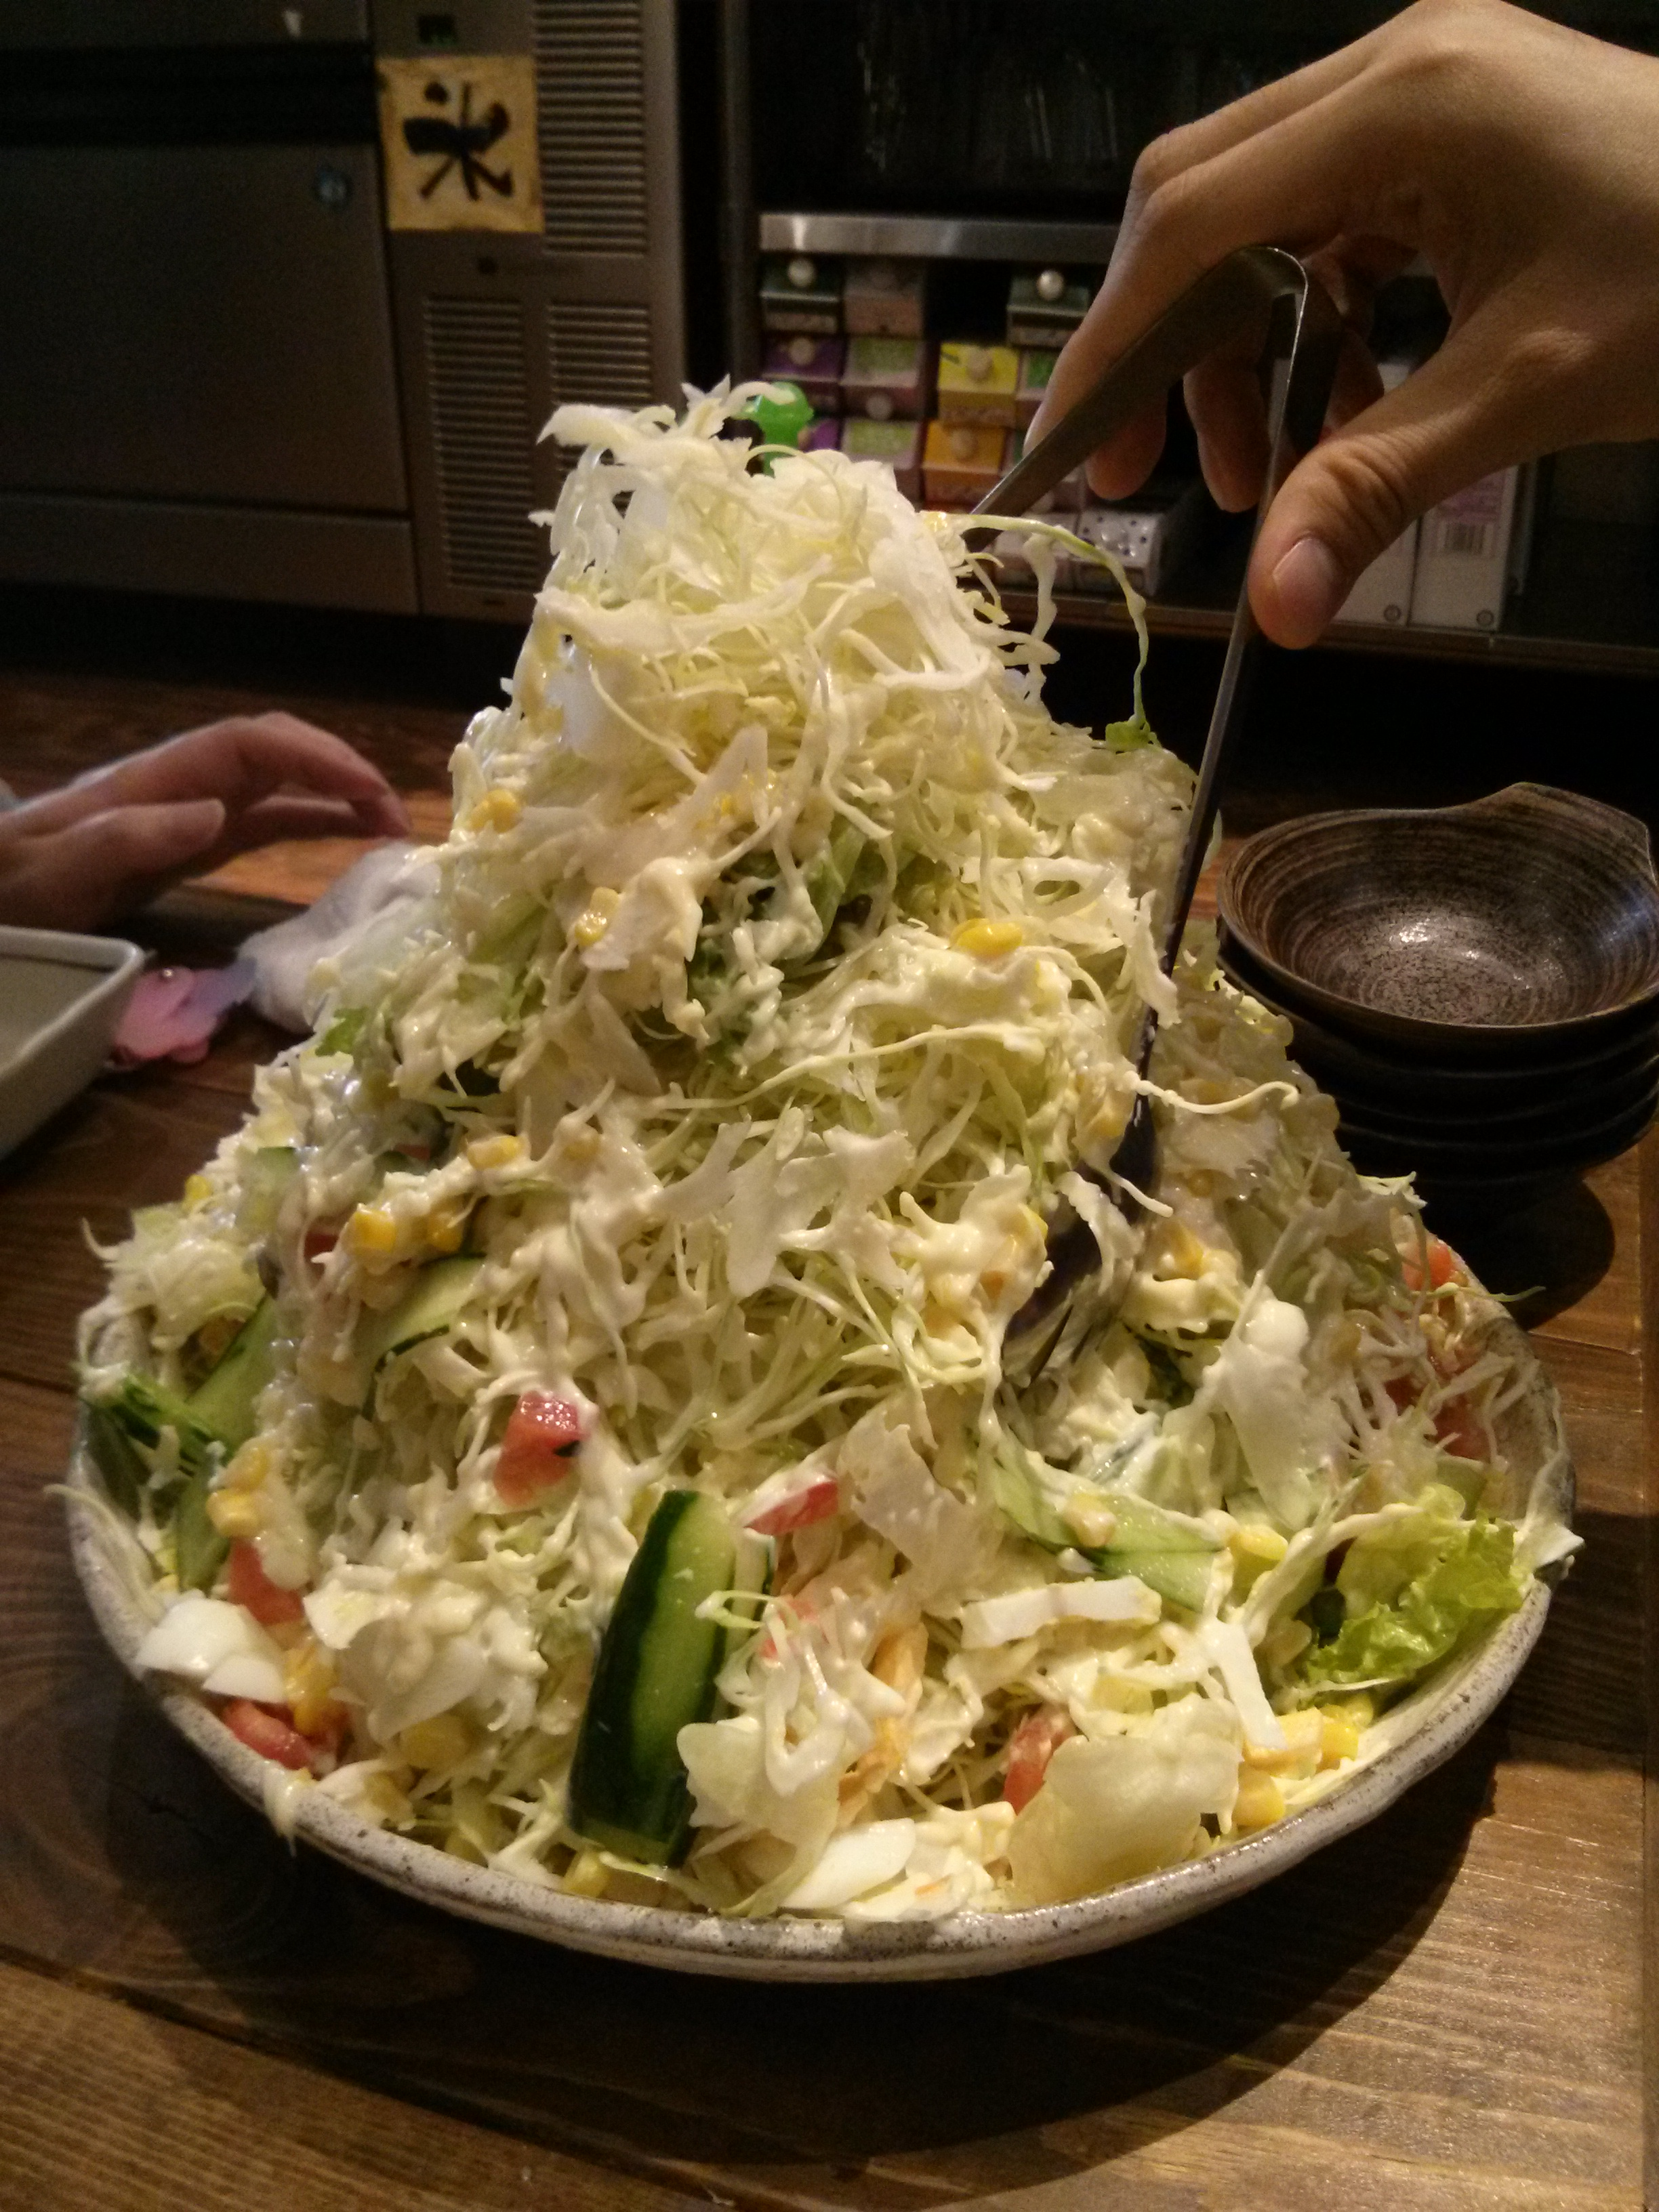
\includegraphics[width=0.5\textwidth]{../images/chikuzen.jpg}
  \caption{デカ盛りサラダとデカ盛り唐揚げでそれだけでお腹いっぱい 激安なのに旨い居酒屋 筑前屋}
\end{figure}

\begin{figure}[H]
  \centering
  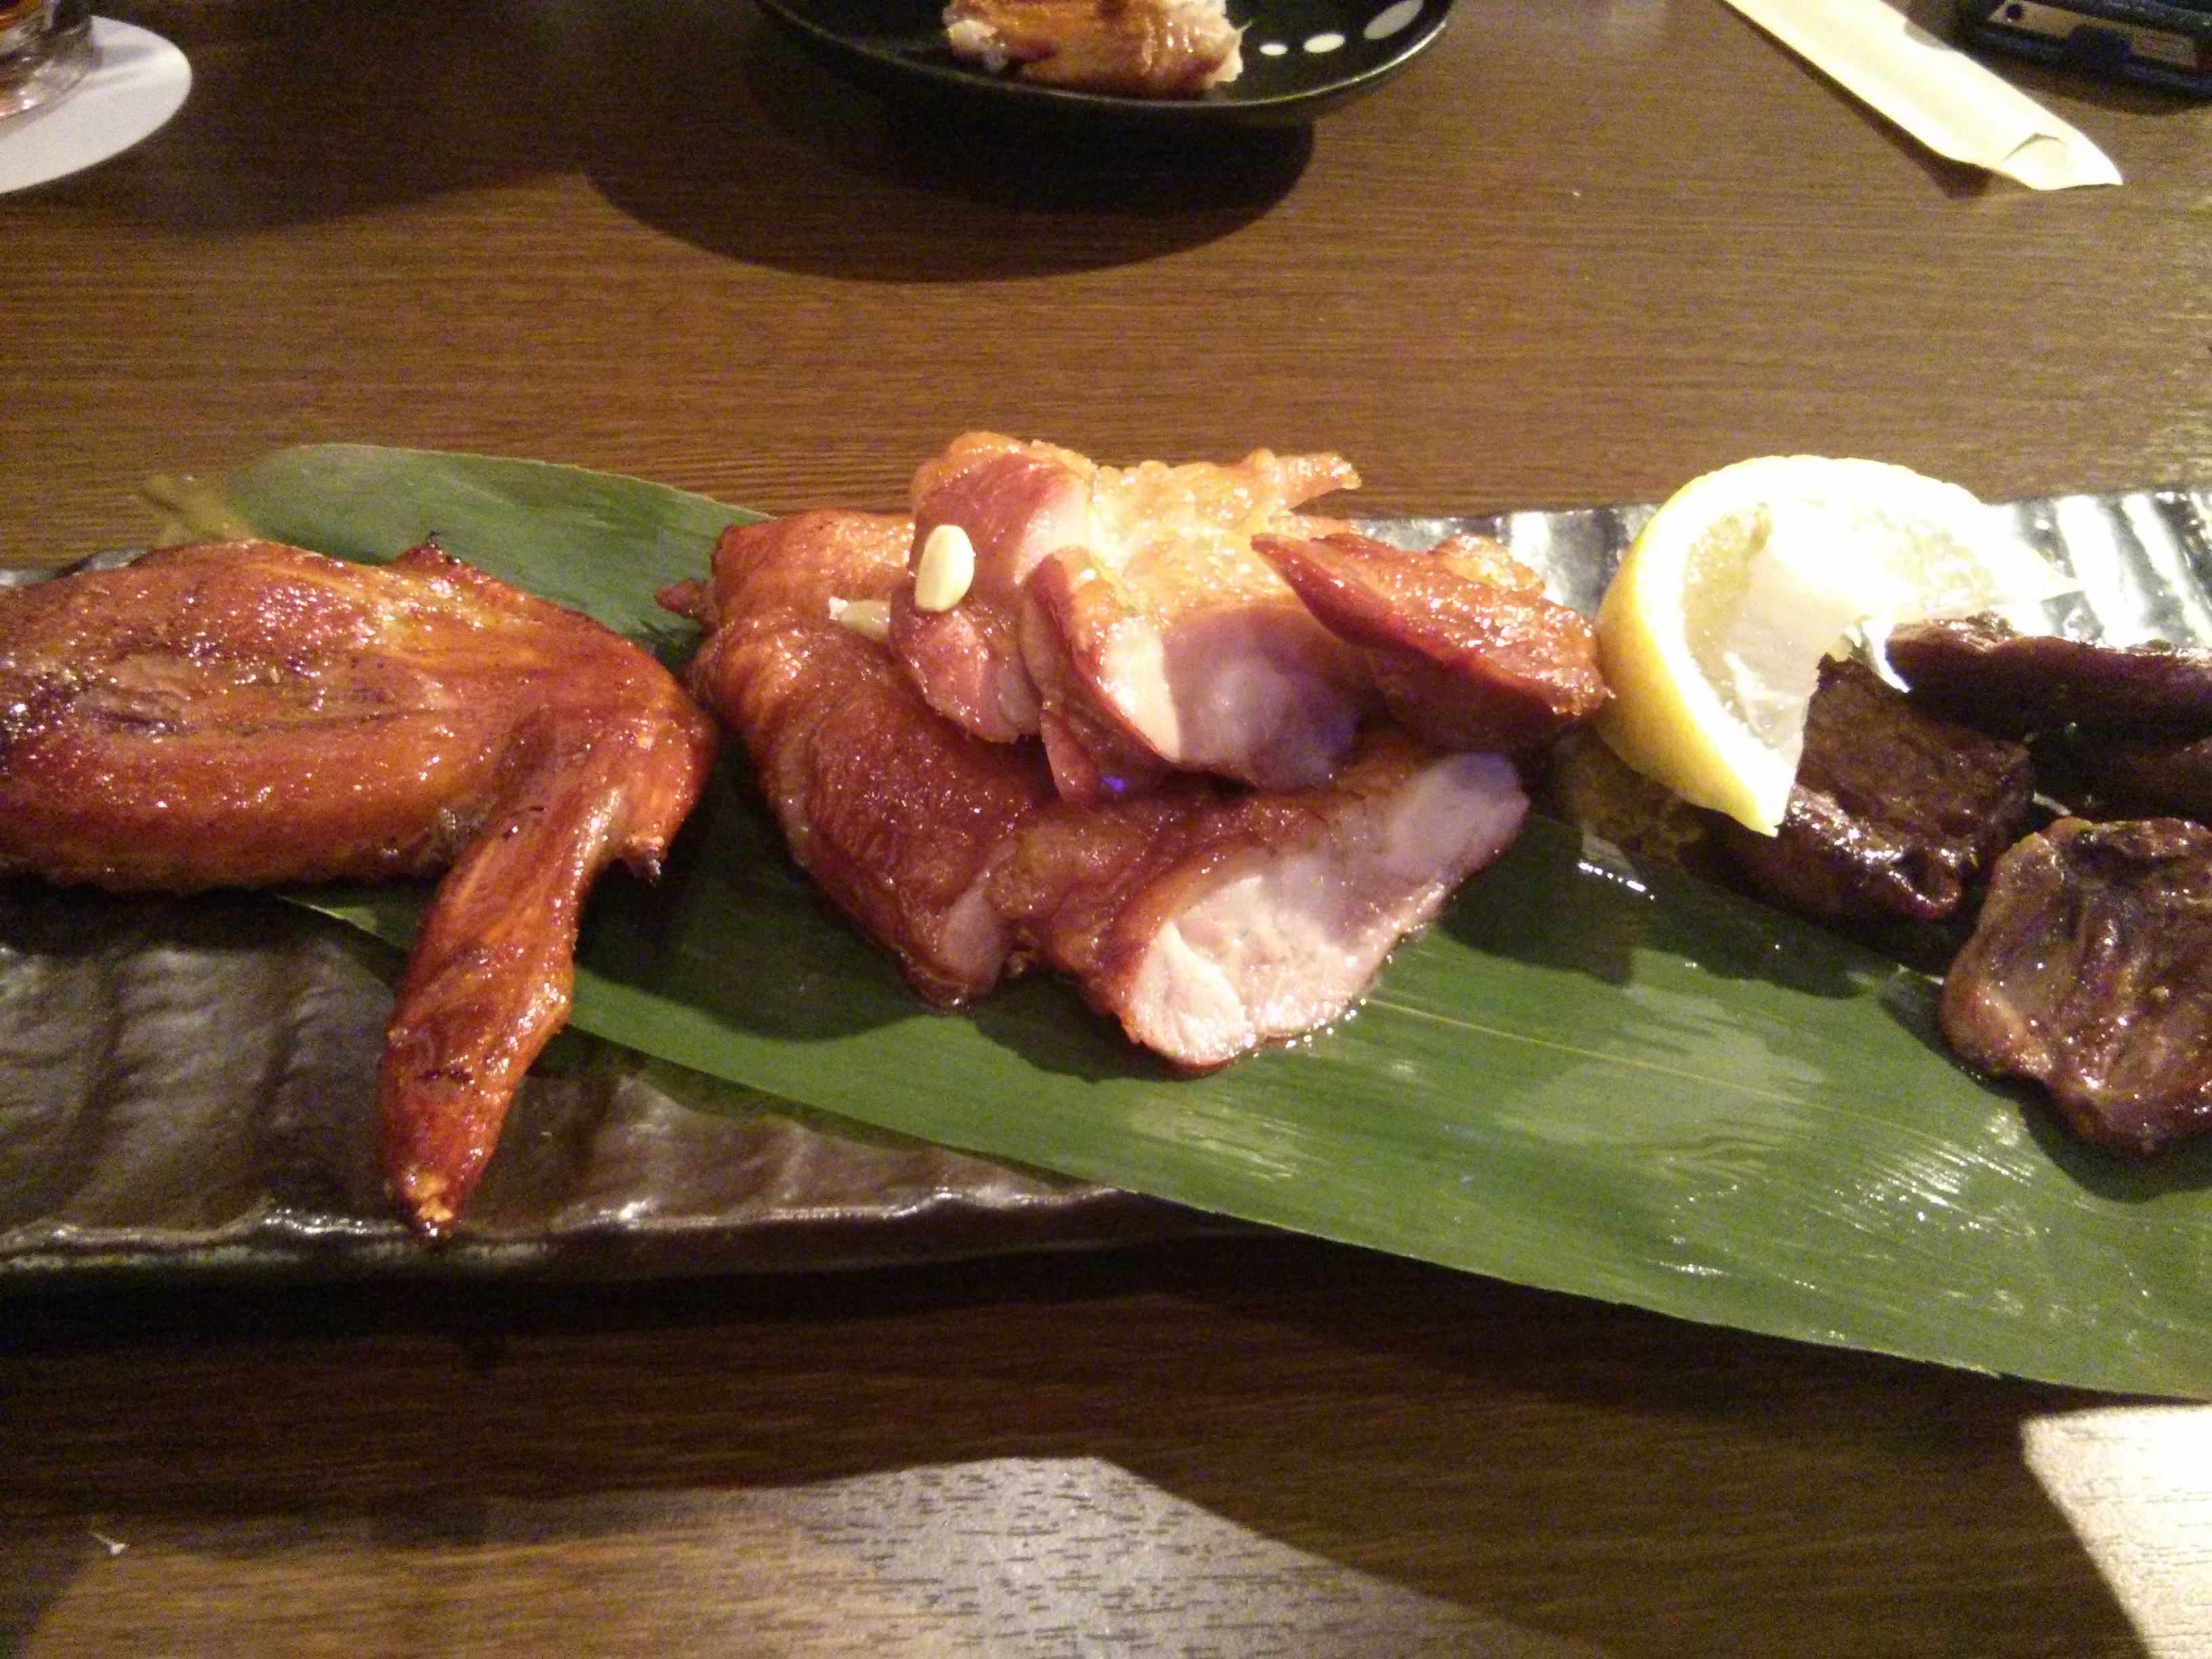
\includegraphics[width=0.5\textwidth]{../images/hanchika.jpg}
  \caption{その場で燻製したものが食べられるハンチカ 燻製ベーコン入のポテトサラダはかなりヤバイ}
\end{figure}

\begin{figure}[H]
  \centering
  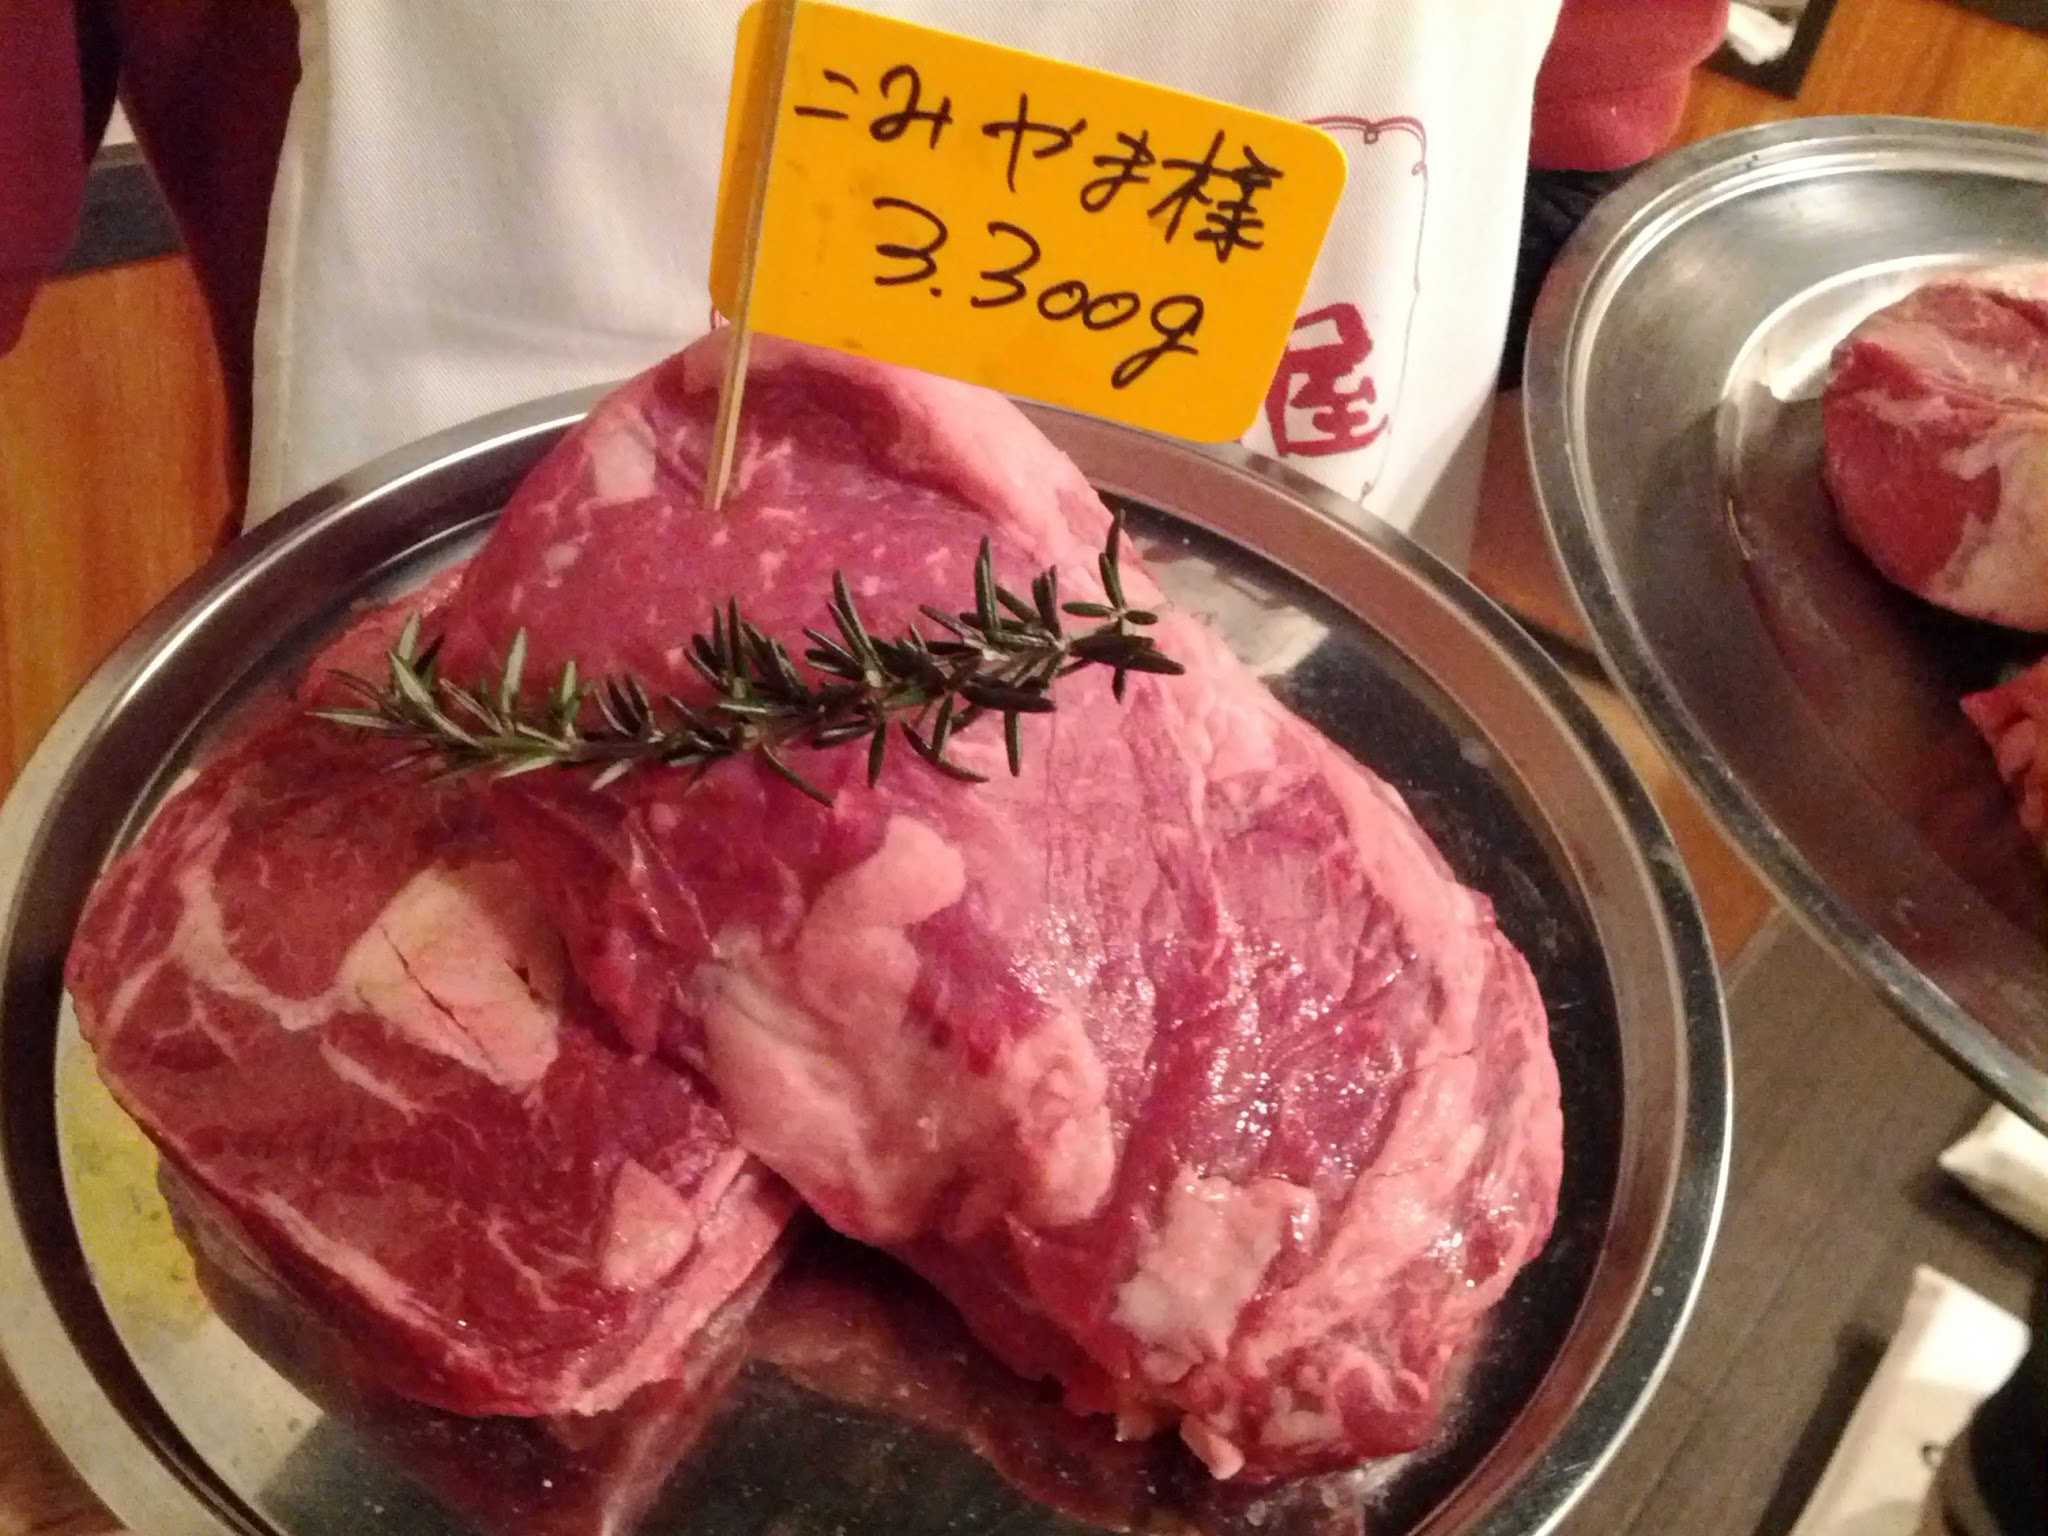
\includegraphics[width=0.5\textwidth]{../images/komatsuya.jpg}
  \caption{ワイルドに肉を喰らうなら小松屋 看板娘のなっちゃんが可愛くて大人気}
\end{figure}

\begin{figure}[H]
  \centering
  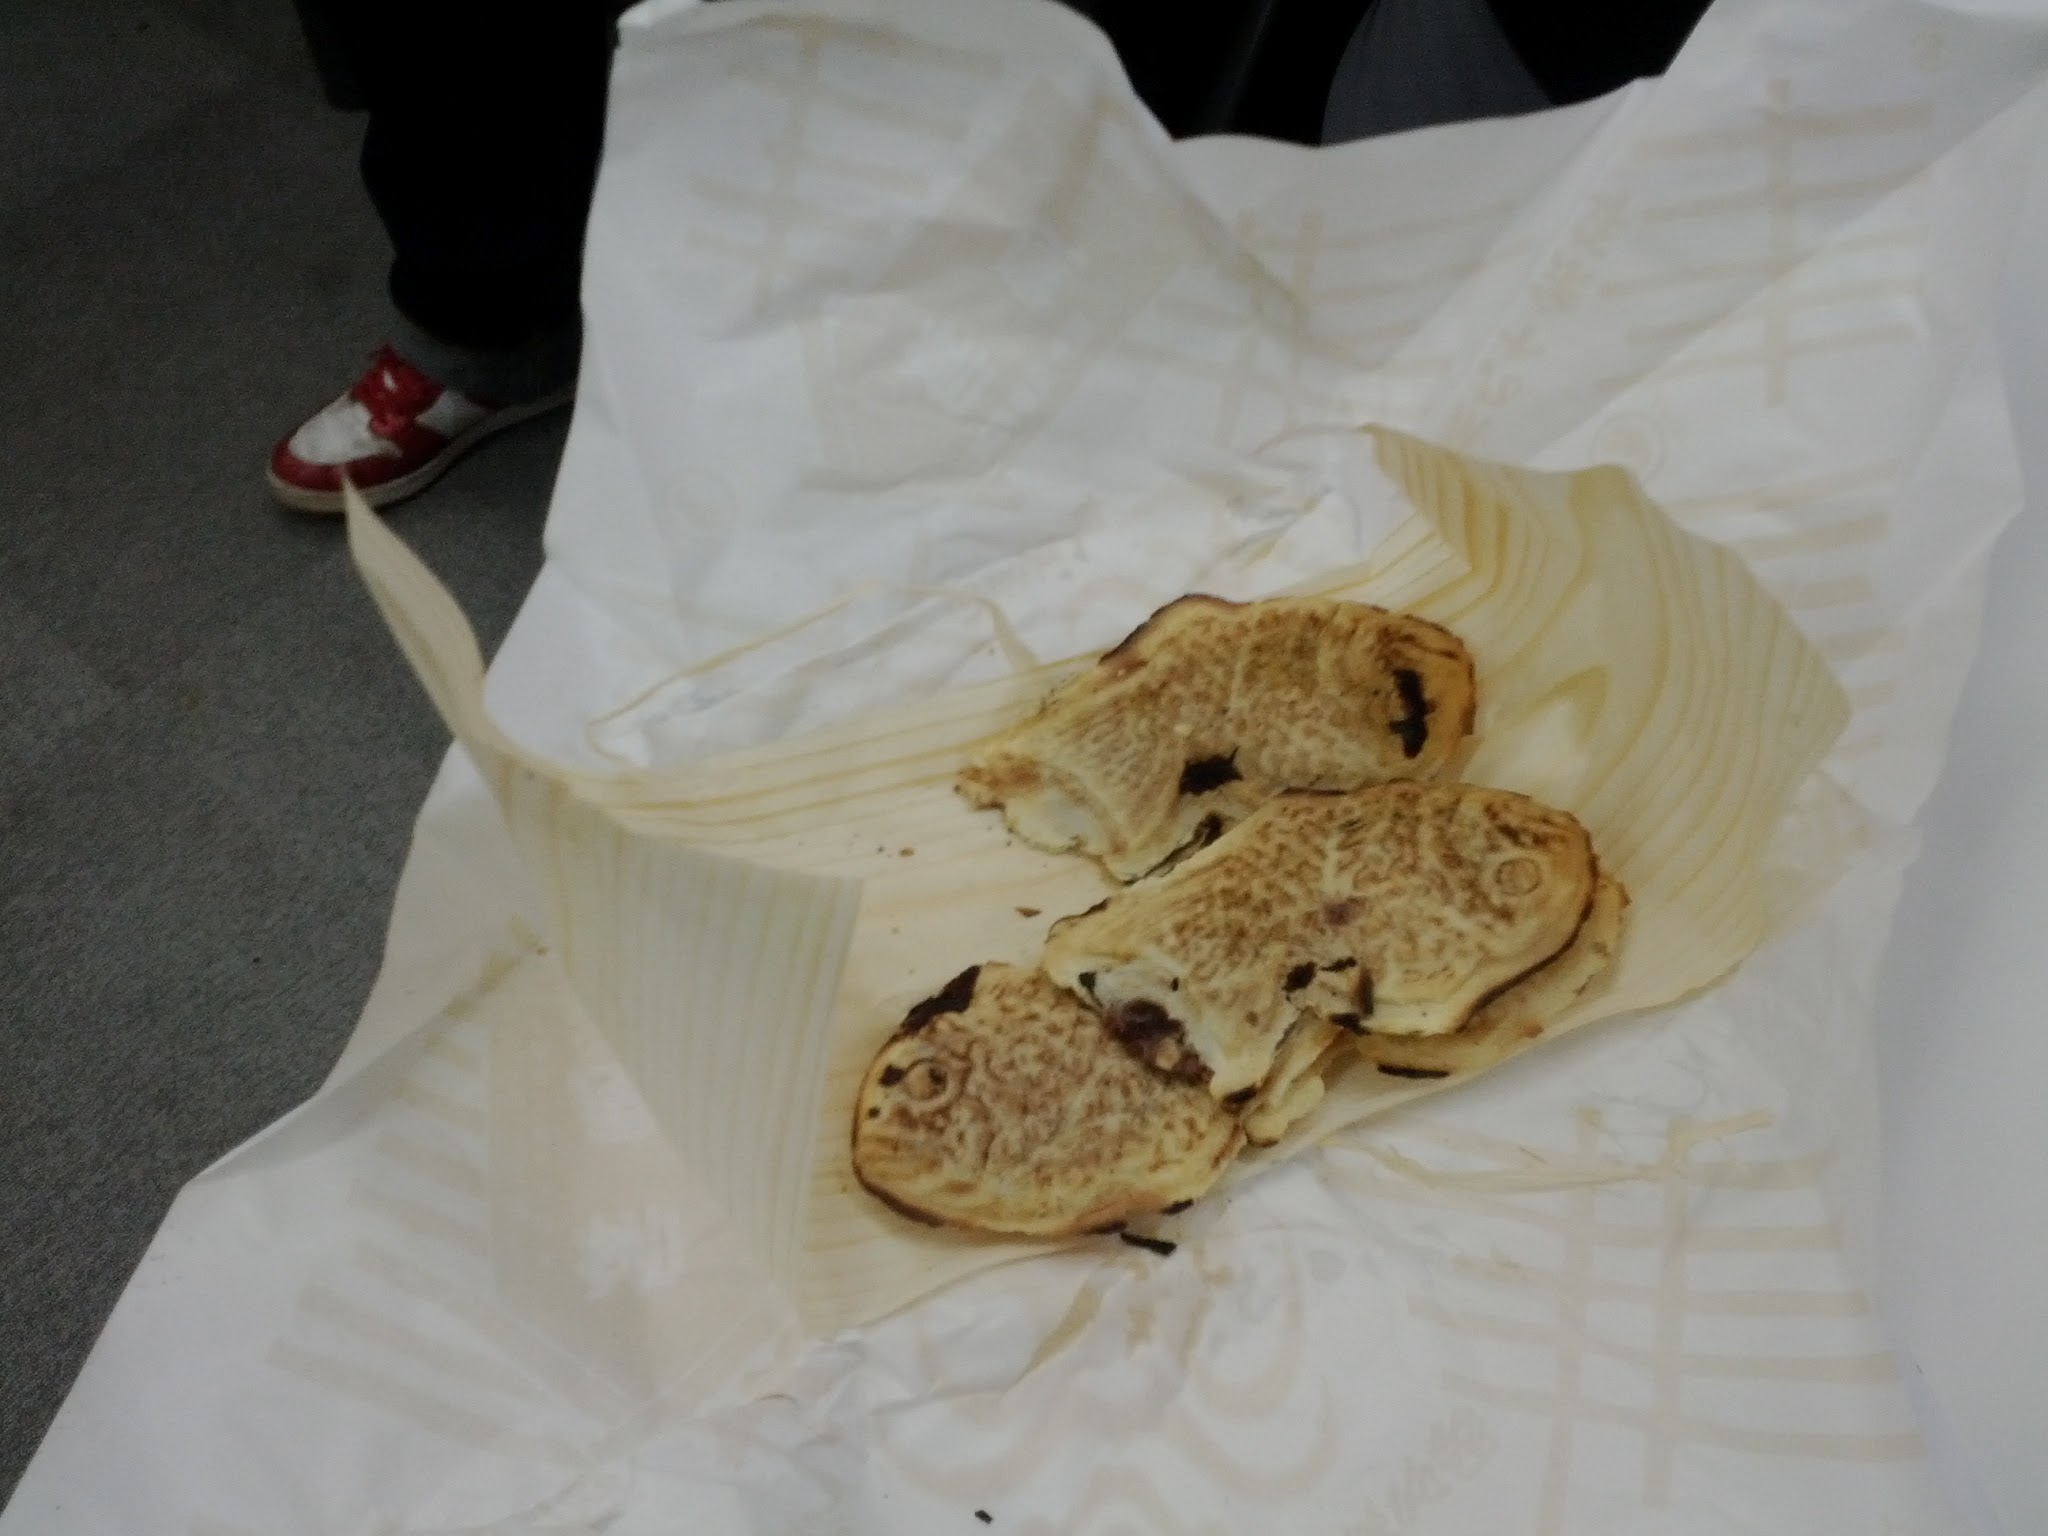
\includegraphics[width=0.5\textwidth]{../images/yanagiya.jpg}
  \caption{柳屋の貴重な天然モノのたい焼き 差し入れとして人気がある いつもすごい行列}
\end{figure}

\subsection{ニコ書を支る飯: 歌舞伎座編}

サブウェイ。
